	\documentclass[14pt]{extarticle}
	
	\usepackage[
	a4paper,
	left=2.5cm,
	right=2.5cm,
	top=2cm,
	bottom=2cm
	]{geometry}
	
	% Sửa lại phần fontspec cho tương thích tốt với XeLaTeX
	\usepackage{fontspec}
	\setmainfont{Times New Roman}
	\usepackage{enumitem}
	\usepackage{graphicx}
	\usepackage{tikz}
	\usetikzlibrary{positioning,arrows.meta,shapes.geometric}
	\usetikzlibrary{calc}
	\usepackage{tikz}
	\usetikzlibrary{positioning}
	
	\renewcommand{\tablename}{Bảng}
	\usepackage{amsmath}
	\usepackage{amssymb}
	\usepackage{hyperref}
	\usepackage{titlesec}
	\usepackage{setspace}
	\usepackage{subcaption}
	\usepackage{tocloft}
	\usepackage{array}
	\usepackage[table,dvipsnames]{xcolor}
	\usepackage{enumitem}
	\usepackage{algorithm}
	\usepackage{algpseudocode}
	\usepackage{listings}
	\usepackage{tcolorbox}
	\usepackage{fontspec}
	\usetikzlibrary{positioning}
	\usepackage{forest}
	\setmonofont{DejaVu Sans Mono}
	
	% ĐÃ XÓA dòng \usepackage{listingsutf8} vì gây lỗi với XeLaTeX
	\renewcommand{\figurename}{Hình }
	\usepackage{booktabs}
	\usepackage{longtable}
	\usepackage{tabularx}
	\usepackage{multirow}
	\renewcommand{\lstlistingname}{Đoạn mã}
	\tcbuselibrary{breakable}
	\usepackage{needspace}
	% Nếu tcolorbox có dùng listings, chỉ khai báo library listings, không khai báo listingsutf8
	\tcbuselibrary{listings} 
	\usepackage{dirtree}
	\usepackage{tikz}
	\usetikzlibrary{positioning}
	% Cấu hình khung chứa cấu trúc thư mục
	\newtcolorbox{folderbox}[1][]{
		colback=gray!5!white,
		colframe=blue!75!black,
		fonttitle=\bfseries,
		title=#1,
		arc=2mm,
		boxrule=0.8pt,
		left=10pt,
		right=10pt,
		top=8pt,
		bottom=8pt
	}
	\lstset{
		language=Python,
		basicstyle=\ttfamily\small,
		keywordstyle=\color{blue},
		commentstyle=\color{ForestGreen},
		stringstyle=\color{red},
		numbers=left,
		numberstyle=\tiny\color{gray},
		stepnumber=1,
		numbersep=3pt,
		xleftmargin=-1pt,
		framexleftmargin=-1.5pt,
		frame=single,
		breaklines=true,
		tabsize=1,
		showstringspaces=false,
		columns=fullflexible,
		keepspaces=true
	}
	
	\setcounter{secnumdepth}{5}
	
	\renewcommand{\thesection}{Chương \arabic{section}.}
	\renewcommand{\thesubsection}{\arabic{section}.\arabic{subsection}.}
	\renewcommand{\thesubsubsection}{\arabic{section}.\arabic{subsection}.\arabic{subsubsection}.}
	\renewcommand{\theparagraph}{\alph{paragraph})}
	
	\algrenewcommand\algorithmicrequire{\textbf{Input:}}
	\algrenewcommand\algorithmicensure{\textbf{Output:}}
	
	\titleformat{\subsection}[hang]
	{\normalfont\large\bfseries}
	{\thesubsection}
	{0.5em}
	{}
	
	\titleformat{\subsubsection}[hang]
	{\normalfont\large\bfseries}
	{\thesubsubsection}
	{0.5em}
	{}
	
	\titleformat{\paragraph}[hang]
	{\normalfont\large\bfseries}
	{\theparagraph}
	{0.5em}
	{}
	
	\setlength{\cftsecnumwidth}{4.9em}
	\setlength{\cftsecindent}{0em}
	
	\setlength{\cftsubsecnumwidth}{2em}
	\setlength{\cftsubsecindent}{1em}
	
	\setlength{\cftsubsubsecnumwidth}{2.5em}
	\setlength{\cftsubsubsecindent}{2em}
	
	\setlength{\cftparaindent}{6em}
	\setlength{\cftparanumwidth}{1.3em}
	
	\titlespacing*{\section}{0pt}{1.5ex plus 1ex minus .2ex}{1ex}
	\titlespacing*{\subsection}{0pt}{1.5ex plus 1ex minus .2ex}{1ex}
	\titlespacing*{\subsubsection}{0pt}{1.5ex plus 1ex minus .2ex}{1ex}
	\titlespacing*{\paragraph}{0pt}{1.5ex plus 1ex minus .2ex}{1ex}
	
	\setlist{
		itemsep=0.2em,
		topsep=1em,
		parsep=0em,
		partopsep=0em
	}
	
	\begin{document}
		
		\onehalfspacing
		
		\begin{titlepage}
			
			\begin{tikzpicture}[remember picture,overlay]
				
				\draw[line width=1.5pt]
				($(current page.north west)+(1.2cm,-1.2cm)$)
				rectangle
				($(current page.south east)+(-1.2cm,1.2cm)$);
				
				\draw[line width=0.8pt]
				($(current page.north west)+(1.5cm,-1.5cm)$)
				rectangle
				($(current page.south east)+(-1.5cm,1.5cm)$);
				
			\end{tikzpicture}
			
			\begin{center}
				
				\vspace*{-1cm}
				
				\textbf{\large ĐẠI HỌC ĐÀ NẴNG}\\
				\textbf{\large TRƯỜNG ĐẠI HỌC SƯ PHẠM}\\
				KHOA TOÁN - TIN
				
				\vspace{1cm}
				
\begin{center}
	
\includegraphics[width=0.45\linewidth]{images/logo}
\end{center}
				
				\vspace{0.8cm}
				
				\textbf{\Large TIỂU LUẬN HỌC PHẦN}\\
			    \vspace{0.3cm}
				\textbf{\large HỌC MÁY NÂNG CAO}
				
				\vspace{1cm}
				
				\textbf{\underline{\textit{ĐỀ TÀI:}}}\\
				\large Triển Khai Mô Hình SVM Phân Loại Hoa Iris
				
			\end{center}
			
			\vspace{1cm}
			
			\begin{tabular}{ll}
				\textbf{Giảng viên hướng dẫn:} & TS. Phan Trần Đức Minh \\[0.4cm]
				\textbf{Họ và tên sinh viên:} & Nguyễn Thị Thanh Thảo \\[0.4cm]
				\textbf{ Mã sinh viên:} & 3110524029
			\end{tabular}
				\vspace{2cm}
			\begin{center}
				{\large Đà Nẵng - 2026}
			\end{center}
			
		\end{titlepage}
		\newpage
			% ================= MỤC LỤC =================
		\renewcommand{\contentsname}{\Large MỤC LỤC}
		\tableofcontents
		\newpage
		\section*{LỜI CẢM ƠN}

		
		\noindent Lời đầu tiên, em xin được bày tỏ lòng biết ơn chân thành và sâu sắc nhất tới TS. Phan Trần Đức Minh, giảng viên hướng dẫn học phần Học Máy Nâng Cao. Trong suốt quá trình học tập và thực hiện đề tài này, Thầy đã luôn tận tình chỉ bảo, truyền đạt những kiến thức chuyên môn quý báu và đưa ra những định hướng quan trọng giúp em tháo gỡ những vướng mắc trong quá trình học tập.\\
		
		\noindent Em cũng xin gửi lời cảm ơn tới Ban Giám hiệu trường Đại học Sư phạm - Đại học Đà Nẵng, cùng các Thầy Cô trong Khoa Toán - Tin đã tạo điều kiện thuận lợi về cơ sở vật chất và môi trường học thuật để em có thể hoàn thành tốt bài tiểu luận này.\\
		
		\noindent Cuối cùng, em đã cùng nhau thảo luận, hỗ trợ và đóng góp ý kiến cùng Thầy và các bạn để hoàn thiện nội dung nghiên cứu. Dù đã có nhiều cố gắng, nhưng do kiến thức còn hạn chế, tiểu luận khó tránh khỏi những thiếu sót. Em rất mong nhận được những ý kiến đóng góp quý báu từ thầy để kiến thức của em ngày càng được hoàn thiện hơn.
	
		\newpage
		\section*{LỜI MỞ ĐẦU}
		\vspace{1.em}
		
		Trong kỷ nguyên chuyển đổi số và Khoa học Dữ liệu hiện nay, việc huấn luyện đạt điểm số tối ưu trong môi trường phòng thí nghiệm (Jupyter Notebook) chỉ là bước đầu tiên của quy trình Học máy. Yếu tố quyết định giá trị thực tiễn của một mô hình AI là khả năng đóng gói tri thức và triển khai (deployment) thành các dịch vụ phần mềm có khả năng tương tác thời gian thực với người dùng.\\  
		
		\noindent Tập dữ liệu hoa Iris (Iris flower dataset) do nhà sinh học Ronald Fisher giới thiệu năm 1936 là tập dữ liệu kinh điển được sử dụng rộng rãi để nghiên cứu các thuật toán phân lớp (Classification). Bài toán đặt ra là xây dựng ranh giới quyết định (Decision Boundary) tối ưu từ 4 thông số hình thái để phân loại chính xác 3 loài hoa Iris.\\
		
		 \noindent  Tiểu luận này trình bày nghiên cứu ứng dụng thuật toán Support Vector Machine (SVM) với Kernel tuyến tính trên tập dữ liệu Iris, áp dụng quy trình tiền xử lý, chia tập dữ liệu Train/Test và kiểm chứng chéo chặt chẽ nhằm tránh hiện tượng Overfitting. Đồng thời, báo cáo trình bày quá trình đóng gói mô hình và xây dựng hệ thống Full-stack Web mang tên \textbf{IRIS BOTANICA AI} dựa trên nền tảng FastAPI kết hợp giao diện HTML5/CSS3/JavaScript tương tác bất đồng bộ.
		 
\subsection*{1. Đặt vấn đề}
	
		 \noindent Trong những năm gần đây, sự phát triển của trí tuệ nhân tạo và học máy (Machine Learning -- ML) đã tạo ra nhiều phương pháp hỗ trợ phân tích dữ liệu và tự động hóa quá trình ra quyết định. Trong lĩnh vực xử lý dữ liệu sinh học và nhận dạng đối tượng, các mô hình học máy có khả năng học các đặc trưng từ dữ liệu mẫu để thực hiện phân loại đối tượng mới một cách nhanh chóng và tự động.\\
	
		 \noindent Bộ dữ liệu hoa Iris là một trong những bộ dữ liệu kinh điển thường được sử dụng trong nghiên cứu và giảng dạy về học máy. Bộ dữ liệu gồm ba loài hoa Iris là Iris Setosa, Iris Versicolor và Iris Virginica, với các đặc trưng gồm chiều dài và chiều rộng của đài hoa (Sepal Length, Sepal Width) và cánh hoa (Petal Length, Petal Width).\\
		 
		 \noindent Với đặc điểm dữ liệu có cấu trúc rõ ràng và số lượng mẫu vừa phải, bộ dữ liệu Iris phù hợp để minh họa quy trình xây dựng một hệ thống phân loại sử dụng học máy.\\
		 
		 \noindent Tuy nhiên, việc xây dựng một mô hình học máy chỉ dừng lại ở bước huấn luyện và đánh giá chưa thể hiện đầy đủ quá trình đưa mô hình vào một hệ thống thực tế. Một hệ thống hoàn chỉnh cần có khả năng tiếp nhận dữ liệu từ người dùng, thực hiện dự đoán thông qua mô hình, trả kết quả trên giao diện web, đồng thời lưu trữ thông tin người dùng và lịch sử dự đoán trong cơ sở dữ liệu. Bên cạnh đó, việc đánh giá và so sánh nhiều mô hình giúp xác định đặc điểm và hiệu quả của từng phương pháp trước khi lựa chọn mô hình để triển khai.\\
		 
		 \noindent Xuất phát từ yêu cầu trên, đề tài ``Xây dựng hệ thống phân loại hoa Iris sử dụng mô hình học máy và triển khai trên nền tảng web'' được thực hiện với mục tiêu xây dựng một quy trình tương đối hoàn chỉnh từ dữ liệu đầu vào đến sản phẩm ứng dụng. Trong đề tài, nhiều mô hình phân loại được huấn luyện và đánh giá dựa trên các chỉ số phù hợp, trong đó mô hình Support Vector Machine (SVM) với kernel tuyến tính được sử dụng để triển khai chức năng dự đoán trên hệ thống.\\
		 
		 \noindent Hệ thống được xây dựng bằng Python và FastAPI, kết hợp với cơ sở dữ liệu để quản lý người dùng, lưu trữ lịch sử dự đoán và thông tin đánh giá mô hình. Giao diện web cho phép người dùng đăng ký, đăng nhập, nhập các thông số của hoa Iris và nhận kết quả phân loại. Kết quả dự đoán đồng thời được lưu vào cơ sở dữ liệu cùng với thời gian thực thi mô hình, qua đó hỗ trợ theo dõi quá trình sử dụng hệ thống.\\
		 
		 \noindent Ngoài môi trường chạy cục bộ, hệ thống còn được triển khai trên nền tảng Render. Trong quá trình triển khai, hệ thống được thiết kế để có thể sử dụng SQL Server trong môi trường cục bộ và PostgreSQL trong môi trường triển khai trực tuyến thông qua biến môi trường \texttt{DATABASE URL}. Điều này giúp hệ thống có khả năng thích ứng với sự khác biệt giữa môi trường phát triển và môi trường triển khai thực tế.\\
		 
\subsection*{2. Mục tiêu đề tài}

\subsubsection*{2.1. Mục tiêu tổng quát}
		 \noindent Xây dựng một hệ thống phân loại hoa Iris dựa trên các mô hình học máy, trong đó thực hiện đầy đủ các bước từ xử lý dữ liệu, huấn luyện và đánh giá mô hình đến triển khai mô hình trên nền tảng web. Hệ thống có khả năng tiếp nhận dữ liệu từ người dùng, thực hiện dự đoán, hiển thị kết quả, quản lý người dùng và lưu trữ lịch sử dự đoán trong cơ sở dữ liệu.\\
		 
\subsubsection*{2.2. Mục tiêu cụ thể}

		  Đề tài tập trung thực hiện các mục tiêu:
		 \begin{itemize}
		 	\item Tìm hiểu bài toán phân loại dữ liệu và các phương pháp học máy phù hợp với bộ dữ liệu Iris.
		 	
		 	\item Khảo sát và xây dựng nhiều mô hình phân loại, thực hiện huấn luyện và đánh giá hiệu năng của các mô hình dựa trên các chỉ số như Accuracy, Precision, Recall và F1-score.
		 	
		 	\item Tìm hiểu mô hình Support Vector Machine (SVM), đặc biệt là SVM sử dụng kernel tuyến tính, và trực quan hóa đường biên quyết định của mô hình.
		 	
		 	\item Lựa chọn mô hình phù hợp để triển khai chức năng dự đoán trên hệ thống web.
		 	
		 	\item Xây dựng API mô hình bằng FastAPI, cho phép hệ thống tiếp nhận các thông số của hoa Iris và trả về kết quả dự đoán.
		 	
		 	\item Xây dựng API kết nối cơ sở dữ liệu nhằm quản lý thông tin người dùng, thông tin mô hình và lịch sử dự đoán.
		 	
		 	\item Xây dựng chức năng đăng ký, đăng nhập và quản lý phiên làm việc của người dùng.
		 	
		 	\item Lưu trữ thông tin đầu vào, kết quả dự đoán, mô hình sử dụng và thời gian thực thi mô hình vào cơ sở dữ liệu.
		 	
		 	\item Xây dựng chức năng xem, xóa, khôi phục, xóa vĩnh viễn lịch sử dự đoán.
		 	
		 	\item Xây dựng giao diện đánh giá mô hình nhằm hiển thị các chỉ số đánh giá và thông tin liên quan đến hiệu năng của các mô hình.
		 	
		 	\item Triển khai hệ thống trên nền tảng Render và kiểm tra khả năng hoạt động của hệ thống trong môi trường trực tuyến.
		 	
		 \end{itemize}
		 
\subsection*{3. Đối tượng và phạm vi nghiên cứu}
	
		 \subsubsection*{3.1. Đối tượng nghiên cứu}
		 
		 \noindent Đối tượng nghiên cứu của đề tài bao gồm các mô hình học máy phục vụ bài toán phân loại hoa Iris, quy trình đánh giá mô hình và phương pháp triển khai mô hình học máy thành một ứng dụng web có khả năng tương tác với người dùng và cơ sở dữ liệu.\\
		 
		 \noindent Cụ thể, đề tài tập trung nghiên cứu các nội dung:
	      		 	 		\vspace{-0.5em}
		 \begin{itemize}
		 	\item Bộ dữ liệu Iris và các đặc trưng được sử dụng để phân loại.
		 	\item Các mô hình học máy phục vụ bài toán phân loại.
		 	\item Mô hình Support Vector Machine với kernel tuyến tính.
		 	\item Các chỉ số đánh giá hiệu năng mô hình.
		 	\item Đường biên quyết định tuyến tính của mô hình SVM.
		 	\item FastAPI và cơ chế xây dựng API cho mô hình học máy.
		 	\item SQLAlchemy và phương pháp kết nối ứng dụng Python với cơ sở dữ liệu.
		 	\item Cơ chế quản lý người dùng và lưu trữ lịch sử dự đoán.
		 \end{itemize}
		 \subsubsection*{3.2. Phạm vi nghiên cứu}
		 
		 \noindent Đề tài được giới hạn trong phạm vi xây dựng hệ thống phân loại ba loài hoa thuộc bộ dữ liệu Iris gồm Iris Setosa, Iris Versicolor và Iris Virginica dựa trên bốn đặc trưng: chiều dài đài hoa, chiều rộng đài hoa, chiều dài cánh hoa và chiều rộng cánh hoa.\\
		 
		 \noindent Về mô hình, đề tài thực hiện huấn luyện và đánh giá nhiều mô hình phân loại nhằm so sánh hiệu năng, sau đó lựa chọn mô hình phù hợp để triển khai chức năng dự đoán trên hệ thống web.\\
		 
		 \noindent Về hệ thống, đề tài tập trung xây dựng giao diện web, API mô hình, API cơ sở dữ liệu, chức năng đăng ký và đăng nhập, lưu trữ lịch sử dự đoán, quản lý lịch sử và hiển thị thông tin đánh giá mô hình.\\
		 
		  \noindent Về môi trường triển khai, hệ thống được phát triển và kiểm thử trên máy tính cá nhân với cơ sở dữ liệu SQL Server, sau đó được triển khai trực tuyến trên nền tảng Render và kết nối với PostgreSQL.\\
		 
\subsection*{4. Phương pháp nghiên cứu}
		 
		  \noindent Để hoàn thành đề tài, các bước công việc được tiến hành như sau:
		   \vspace{-0.5em}
		   \begin{enumerate}[leftmargin=*]
		   	\item \textbf{Đọc và tổng hợp tài liệu:} Tìm hiểu lý thuyết về cách thuật toán SVM tính toán ranh giới phân loại và cách kết nối mô hình học máy với giao diện trang web.
		   	\item \textbf{Xử lý dữ liệu và chạy mô hình:} Quan sát đặc điểm các con số trong bộ dữ liệu Iris, sau đó viết chương trình cho máy tính học và tìm ra bộ quy tắc phân loại tốt nhất.
		   	\item \textbf{Thử nghiệm và kiểm tra độ chính xác:}
		   		 \vspace{-1em}
		   	\begin{itemize}
		   		\item Tách riêng một phần dữ liệu không cho mô hình biết trước để làm bài kiểm tra.
		   		\item Chia nhỏ dữ liệu thành 5 phần, cho mô hình học 4 phần và thi thử trên phần còn lại, lặp lại 5 lần để đảm bảo mô hình đoán chuẩn xác thật sự chứ không phải do may mắn.
		   	\end{itemize}
		   	 \vspace{-1em}
		   	\item \textbf{Xây dựng ứng dụng trang web:} Thiết kế giao diện cho người dùng nhập số liệu, kết nối với phần xử lý ngầm để khi bấm nút, trang web sẽ hiển thị ngay tên và hình ảnh loài hoa tương ứng.
		   \end{enumerate}
		   \newpage
		   
\subsection*{ 5. Nội dung thực hiện}
thực
		   
		   Để đạt được các mục tiêu đề ra, đề tài được thực hiện theo các nội dung chính sau:
		   
		   \begin{enumerate}
		   	\item Khảo sát bài toán và tìm hiểu bộ dữ liệu Iris.
		   	
		   	\item Phân tích dữ liệu, xác định các đặc trưng đầu vào và biến mục tiêu.
		   	
		   	\item Tiền xử lý và phân chia dữ liệu thành tập huấn luyện và tập kiểm thử.
		   	
		   	\item Xây dựng nhiều mô hình phân loại và tiến hành huấn luyện trên tập dữ liệu.
		   	
		   	\item Đánh giá và so sánh các mô hình dựa trên Accuracy, Precision, Recall, F1-score và ma trận nhầm lẫn.
		   	
		   	\item Phân tích mô hình SVM với kernel tuyến tính và trực quan hóa đường biên quyết định.
		   	
		   	\item Lưu mô hình đã huấn luyện để sử dụng trong quá trình triển khai ứng dụng.
		   	
		   	\item Xây dựng API bằng FastAPI để kết nối mô hình học máy với giao diện web.
		   	
		   	\item Xây dựng cơ sở dữ liệu phục vụ quản lý người dùng, thông tin mô hình và lịch sử dự đoán.
		   	
		   	\item Xây dựng chức năng đăng ký, đăng nhập và quản lý phiên người dùng.
		   	
		   	\item Xây dựng chức năng dự đoán hoa Iris trên giao diện web và lưu kết quả vào cơ sở dữ liệu.
		   	
		   	\item Bổ sung thông tin thời gian thực thi mô hình nhằm theo dõi hiệu năng của quá trình dự đoán.
		   	
		   	\item Xây dựng chức năng xem, xóa, khôi phục và xóa vĩnh viễn lịch sử dự đoán.
		   	
		   	\item Xây dựng trang hiển thị kết quả đánh giá các mô hình.
		   	
		   	\item Kiểm thử hệ thống trong môi trường cục bộ và triển khai hệ thống trên nền tảng Render.
		   	
		   \end{enumerate}
		   
		   Quy trình thực hiện có thể được khái quát theo chuỗi:
		   
		   \begin{center}
		   	\textbf{Dữ liệu}
		   	$\rightarrow$
		   	\textbf{Tiền xử lý}
		   	$\rightarrow$
		   	\textbf{Huấn luyện}
		   	$\rightarrow$
		   	\textbf{Đánh giá}
		   	$\rightarrow$
		   	\textbf{Triển khai mô hình}
		   	$\rightarrow$
		   	\textbf{API}
		   	$\rightarrow$
		   	\textbf{CSDL}
		   	$\rightarrow$
		   	\textbf{Web}
		   	$\rightarrow$
		   	\textbf{Triển khai trực tuyến}.
		   \end{center}
		   
		   
\subsection*{6. Nội dung nghiên cứu}
		 \noindent Nội dung báo cáo được chia thành các phần rõ ràng như sau:
	
	\begin{itemize}
	
		\item \textbf{Chương 1 -- Cơ sở lý thuyết:} Trình bày các kiến thức nền tảng liên quan đến học máy, bộ dữ liệu Iris, các mô hình phân loại, các chỉ số đánh giá và cơ sở lý thuyết về SVM với đường biên quyết định tuyến tính.
		
		\item \textbf{Chương 2 -- Phân tích và xây dựng mô hình:} Trình bày quá trình xử lý dữ liệu, huấn luyện nhiều mô hình, đánh giá và so sánh kết quả, đồng thời phân tích đường tuyến tính của mô hình SVM được lựa chọn.
		
		\item \textbf{Chương 3 -- Xây dựng hệ thống web:} Trình bày quá trình chuyển mô hình học máy thành hệ thống ứng dụng, bao gồm xây dựng API mô hình, API cơ sở dữ liệu, quản lý người dùng, lưu trữ lịch sử, đo thời gian thực thi và xây dựng giao diện web.
		
		\item \textbf{Chương 4 -- Kiểm thử và triển khai:} Trình bày các trường hợp kiểm thử, kết quả hoạt động của hệ thống, quá trình triển khai trên Render và một số vấn đề phát sinh trong quá trình phát triển cùng cách khắc phục.
		
		\item \textbf{Kết luận và hướng phát triển:} Tổng kết kết quả đạt được, những hạn chế còn tồn tại và đề xuất các hướng phát triển hệ thống trong tương lai.
		
		\item \textbf{Phụ lục:} Cung cấp các mã nguồn và tài liệu kỹ thuật cần thiết để tham khảo.
		
	\end{itemize}
		 \newpage
		 
		 
		 
		 
		 \section{CƠ SỞ LÝ THUYẾT VỀ MACHINE LEARNING}
		 \subsection{Tổng quan về học máy }
		 \noindent Học máy (Machine Learning) là một lĩnh vực của trí tuệ nhân tạo, tập trung vào việc xây dựng các phương pháp cho phép máy tính học các quy luật hoặc mối quan hệ từ dữ liệu để thực hiện dự đoán hoặc đưa ra quyết định trên những dữ liệu mới.\\
		 
		\noindent  Khác với cách lập trình truyền thống, trong đó các quy tắc xử lý được xây dựng trực tiếp bởi người lập trình, học máy sử dụng dữ liệu làm cơ sở để mô hình tự tìm ra mối quan hệ giữa các biến đầu vào và kết quả đầu ra.\\
		 
		 \noindent Một hệ thống học máy thường bao gồm dữ liệu đầu vào, đặc trưng, biến mục tiêu, mô hình học máy và quá trình đánh giá. Với bài toán phân loại hoa Iris trong đề tài, các đặc trưng đầu vào là các thông số đo của hoa, trong khi biến mục tiêu là loài hoa tương ứng.\\
		 
		 \noindent Có thể biểu diễn một bài toán học có giám sát tổng quát như sau:
		 
		 \begin{equation*}
		 	f: X \rightarrow Y
		 \end{equation*}
		 
		\noindent trong đó $X$ là không gian các đặc trưng đầu vào, $Y$ là tập các nhãn đầu ra và $f$ là hàm được mô hình học máy học từ dữ liệu huấn luyện. Trong đề tài này, bài toán được xây dựng theo phương pháp học có giám sát
		 (Supervised Learning), bởi dữ liệu huấn luyện đã có sẵn nhãn tương ứng với
		 ba loài hoa Iris.
		 
		 \subsection{Bài toán phân loại }
		 
	 	\noindent Phân loại (Classification) là một bài toán học máy có giám sát, trong đó mục tiêu là xây dựng một mô hình có khả năng gán một đối tượng mới vào một trong các lớp đã được xác định trước.\\
		 \newpage
		 \noindent Với tập dữ liệu huấn luyện:
		 
		 \begin{equation*}
		 	D = \{(x_i,y_i)\}_{i=1}^{n}
		 \end{equation*}
		 
		 	\noindent trong đó $x_i$ là vector đặc trưng của mẫu thứ $i$, $y_i$ là nhãn tương ứng
		 và $n$ là số lượng mẫu.
		 
		\noindent Mục tiêu của mô hình là học một hàm:
		 
		 \begin{equation*}
		 	f(x) = y
		 \end{equation*}
		 
		 	\noindent để dự đoán nhãn cho một mẫu dữ liệu chưa xuất hiện trong quá trình huấn luyện. Trong đề tài IRIS BOTANICA AI, bài toán là phân loại đa lớp với ba lớp:
		 
		 \begin{itemize}
		 	\item Iris Setosa;
		 	\item Iris Versicolor;
		 	\item Iris Virginica.
		 \end{itemize}
		 
		 	\noindent Mỗi mẫu dữ liệu được biểu diễn bởi bốn đặc trưng:
		 
		 \begin{itemize}
		 	\item Chiều dài đài hoa (Sepal Length);
		 	\item Chiều rộng đài hoa (Sepal Width);
		 	\item Chiều dài cánh hoa (Petal Length);
		 	\item Chiều rộng cánh hoa (Petal Width).
		 \end{itemize}
		 
			\noindent Sau khi mô hình được huấn luyện, bốn giá trị này được sử dụng làm đầu vào để dự đoán loài hoa tương ứng.
			
		 \subsection{ Bộ dữ liệu Iris }
		 	\noindent Bộ dữ liệu Iris là một trong những bộ dữ liệu kinh điển được sử dụng rộng rãi trong nghiên cứu và giảng dạy về học máy. Dữ liệu mô tả ba loài hoa Iris dựa trên các đặc trưng hình thái của hoa.
		 
		 	\noindent Bộ dữ liệu gồm 150 mẫu, được chia thành ba lớp tương ứng với ba loài hoa. Mỗi mẫu có bốn đặc trưng định lượng.
		 
		 \begin{table}[H]
		 	\centering
		 	\caption{Các đặc trưng của bộ dữ liệu Iris}
		 	\label{tab:iris-features}
		 	\begin{tabular}{p{4cm} p{4cm} p{5cm}}
		 		\toprule
		 		\textbf{Đặc trưng} & \textbf{Đơn vị} & \textbf{Ý nghĩa} \\
		 		\midrule
		 		Sepal Length & cm & Chiều dài đài hoa \\
		 		Sepal Width & cm & Chiều rộng đài hoa \\
		 		Petal Length & cm & Chiều dài cánh hoa \\
		 		Petal Width & cm & Chiều rộng cánh hoa \\
		 		\bottomrule
		 	\end{tabular}
		 \end{table}
		 
			\noindent Biến mục tiêu của bài toán là loài hoa. Ba lớp được mã hóa thành các nhãn khác nhau để thuận tiện cho quá trình huấn luyện mô hình.
		 
		 \begin{table}[H]
		 	\centering
		 	\caption{Các lớp của bộ dữ liệu Iris}
		 	\label{tab:iris-classes}
		 	\begin{tabular}{c l}
		 		\toprule
		 		\textbf{Nhãn} & \textbf{Loài hoa} \\
		 		\midrule
		 		0 & Iris Setosa \\
		 		1 & Iris Versicolor \\
		 		2 & Iris Virginica \\
		 		\bottomrule
		 	\end{tabular}
		 \end{table}
		 \begin{figure}[H]
		 	\centering
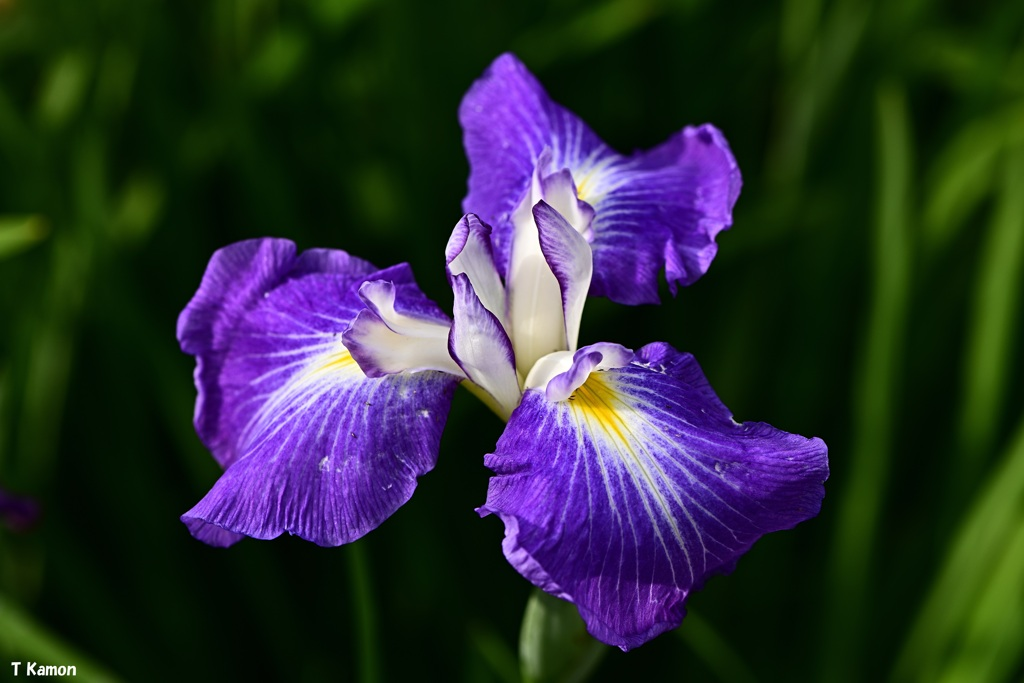
\includegraphics[width=0.30\textwidth]{images/SETOSA}
		 	\hfill
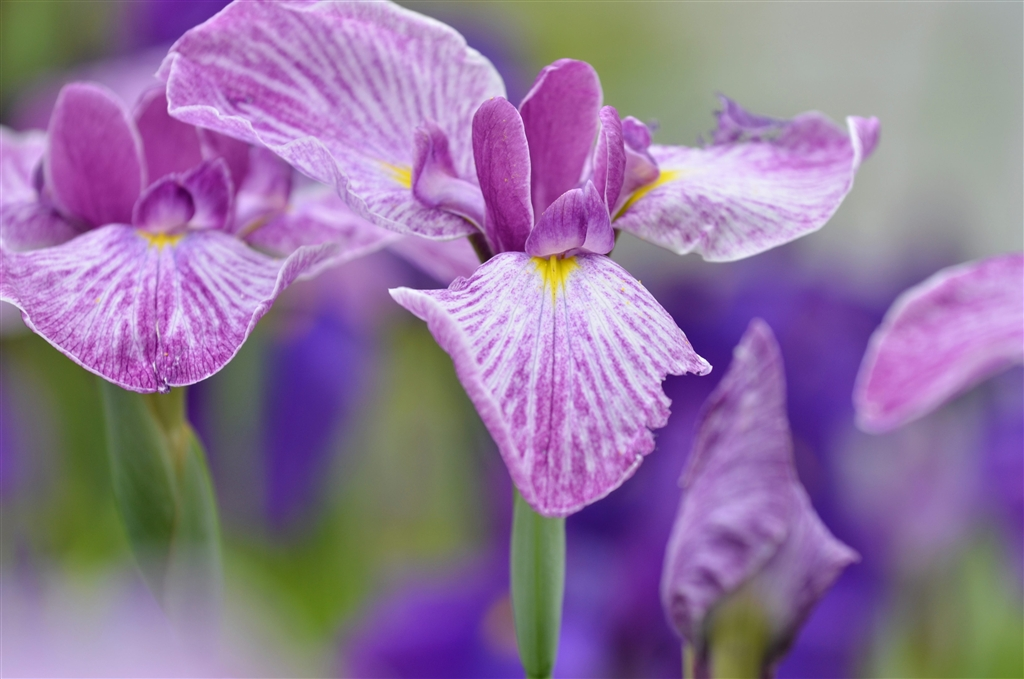
\includegraphics[width=0.30\textwidth]{images/VERSICOLOR_v2}
		 	\hfill
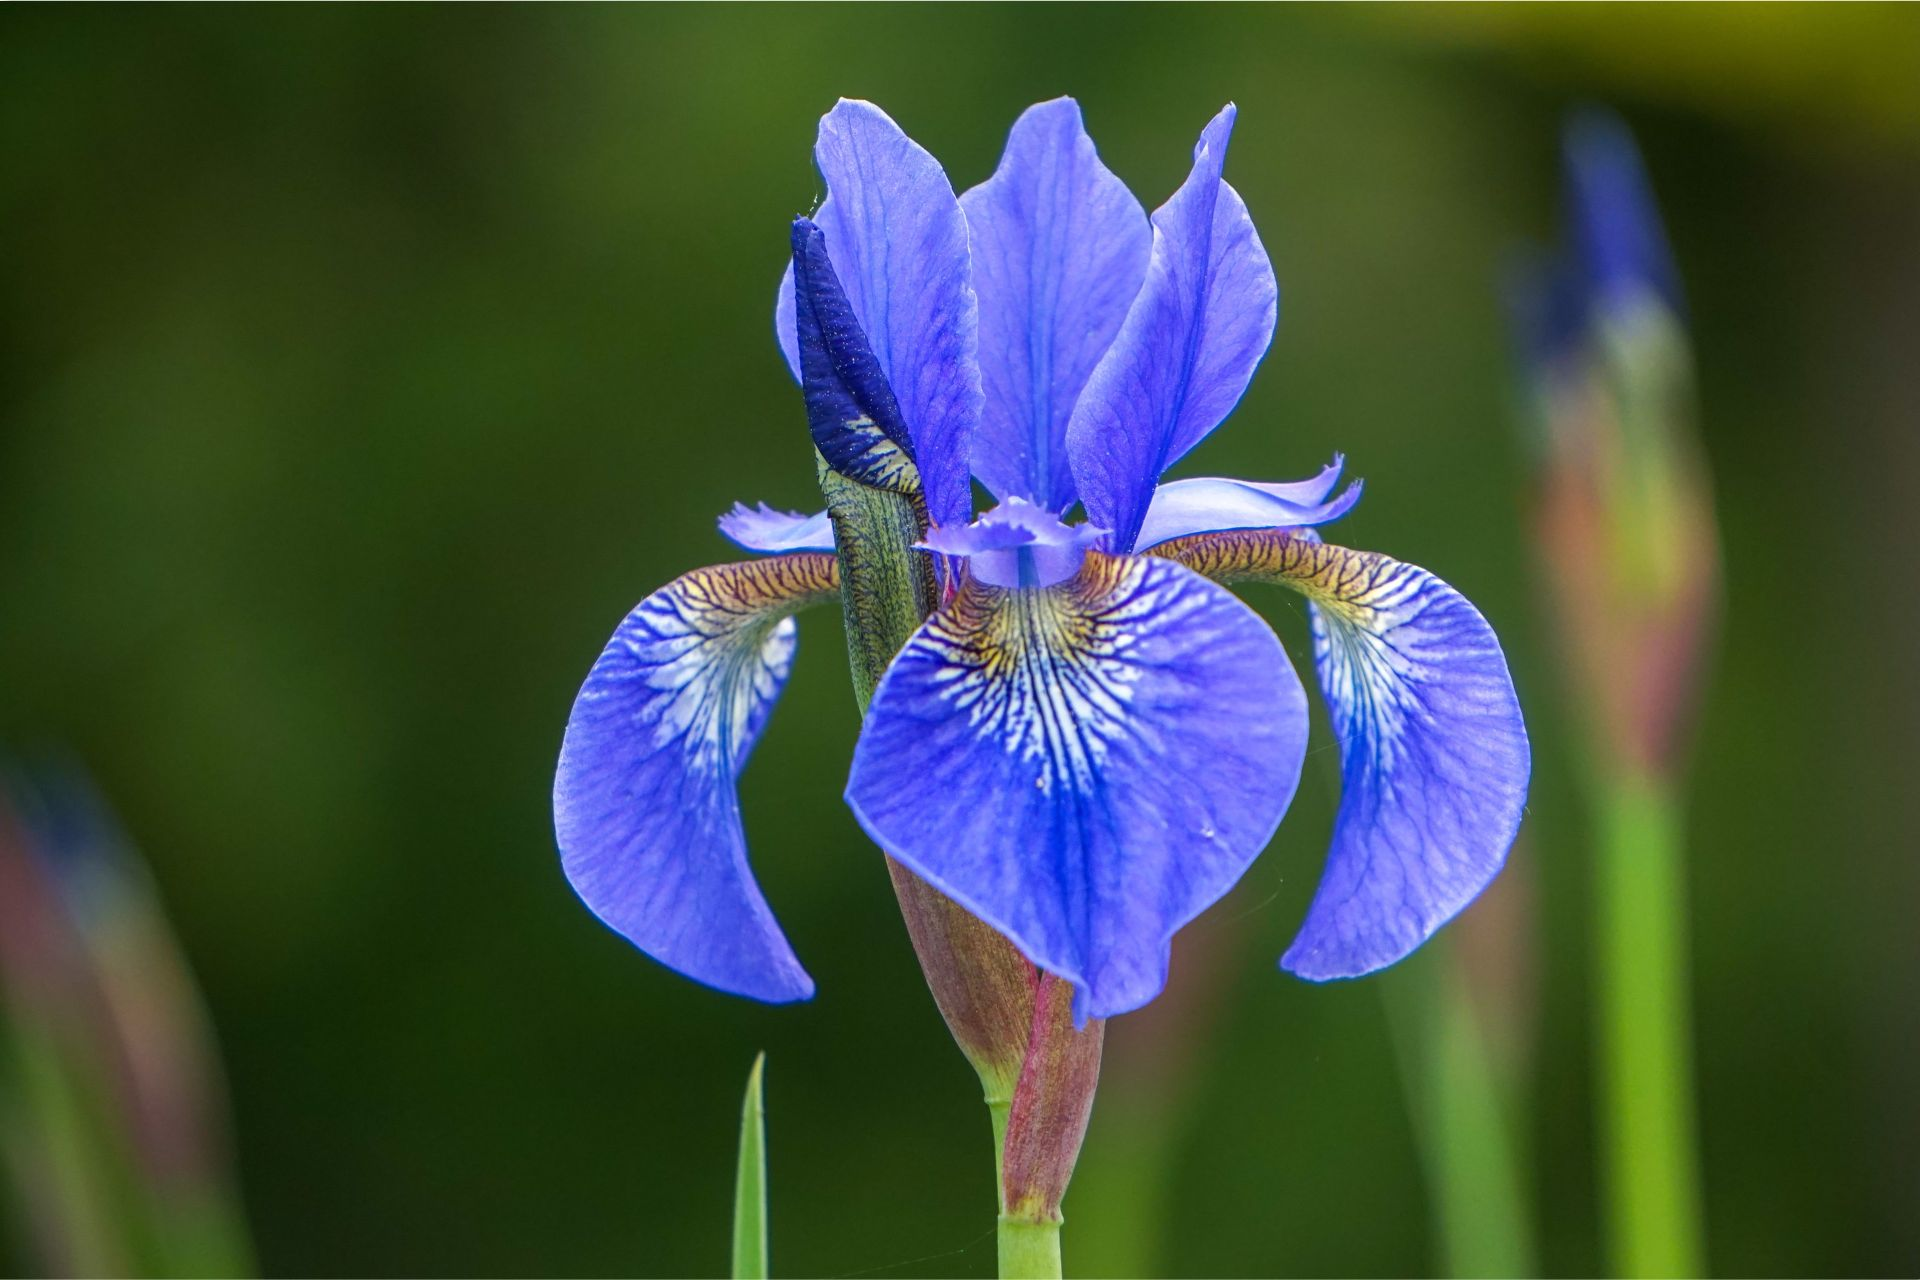
\includegraphics[width=0.30\textwidth]{images/VIRGINICA_v2}
	\caption{Các giao diện của hoa diên vĩ Iris}
	\label{fig:ba-giao-dien}
	\end{figure}
		 \subsection{Tiền xử lý và chia dữ liệu }
		 \noindent Trước khi huấn luyện mô hình, dữ liệu cần được tổ chức thành tập đặc trưng đầu vào và tập nhãn mục tiêu. Trong bài toán Iris, ma trận đặc trưng $X$ gồm bốn thuộc tính đo lường của hoa, trong khi vector $y$ chứa nhãn của từng mẫu.\\
		 
		 \noindent Dữ liệu được chia thành hai tập:
		 
		 \begin{itemize}
		 	\item \textbf{Tập huấn luyện (Training Set):} được sử dụng để mô hình
		 	học các mối quan hệ giữa đặc trưng và nhãn.
		 	
		 	\item \textbf{Tập kiểm thử (Test Set):} được sử dụng để đánh giá khả năng
		 	dự đoán của mô hình trên những dữ liệu không được sử dụng trong quá trình
		 	huấn luyện.
		 \end{itemize}
		 
		\noindent Trong đề tài, dữ liệu được chia theo tỷ lệ 80\% cho tập huấn luyện và 20\% cho tập kiểm thử. Tham số \texttt{random\_state=42} được sử dụng nhằm đảm bảo kết quả chia dữ liệu có thể được tái lập.\\
		 
		 \noindent Ngoài ra, tham số \texttt{stratify=y} được sử dụng để duy trì tỷ lệ tương đối của các lớp trong cả tập huấn luyện và tập kiểm thử.\\
		 
		 \noindent Với 150 mẫu dữ liệu Iris, quá trình chia dữ liệu tạo ra:
		 \vspace{-0.5em}
		 \begin{itemize}
		 	\item 120 mẫu cho tập huấn luyện;
		 	\item 30 mẫu cho tập kiểm thử.
		 \end{itemize}
		 \subsection{Mô hình học máy}
		 \subsubsection{Support Vector Machine - SVM }
			\noindent  Support Vector Machine (SVM) là một thuật toán học có giám sát được sử dụng cho các bài toán phân loại và hồi quy. Ý tưởng chính của SVM là tìm một siêu phẳng có khả năng phân tách các lớp dữ liệu với khoảng cách biên lớn nhất.
		 
		 	\noindent  Đối với trường hợp phân loại tuyến tính, siêu phẳng có thể được biểu diễn bởi:
		 
		 \begin{equation*}
		 	w^T x + b = 0
		 \end{equation*}
		 
		 	\noindent trong đó $w$ là vector trọng số, $x$ là vector đặc trưng và $b$ là hệ số
		 bias.
		 
		 	\noindent SVM tìm siêu phẳng sao cho các mẫu thuộc các lớp khác nhau được phân tách với biên lớn nhất. Các điểm dữ liệu nằm gần biên phân lớp có vai trò quan trọng trong việc xác định vị trí của siêu phẳng và được gọi là các Support Vectors.
		 
		 	\noindent Trong đề tài, mô hình SVM được xây dựng với kernel tuyến tính
		 (\texttt{kernel="linear"}). Việc sử dụng kernel tuyến tính phù hợp với mục
		 tiêu phân tích đường phân lớp tuyến tính và giúp mô hình có thể được
		 trực quan hóa rõ ràng hơn.
		 \newpage
		\noindent  Với bài toán đa lớp gồm ba loài hoa Iris, thư viện Scikit-learn thực hiện việc mở rộng bài toán nhị phân của SVM thành bài toán phân loại đa lớp.\\
		
		 \subsubsection{Logistic Regression}
		 
			\noindent Logistic Regression là một thuật toán học có giám sát thường được sử dụng cho các bài toán phân loại. Mô hình ước lượng xác suất một mẫu thuộc về một lớp dựa trên tổ hợp tuyến tính của các đặc trưng đầu vào.
		 
		 	\noindent Đối với bài toán nhị phân, xác suất được mô hình hóa thông qua hàm sigmoid:
		 
		 \begin{equation*}
		 	\sigma(z) = \frac{1}{1+e^{-z}}
		 \end{equation*}
		 
		 với:
		 
		 \begin{equation*}
		 	z = w^T x + b
		 \end{equation*}
		 
			\noindent  Trong bài toán Iris, Logistic Regression có thể được mở rộng để xử lý phân loại đa lớp. Mô hình được sử dụng như một phương pháp tham chiếu để so sánh với SVM và các mô hình khác trong đề tài.\\
			\subsubsection{K-Nearest Neighbors}
			
				\noindent K-Nearest Neighbors (KNN) là phương pháp phân loại dựa trên khoảng cách giữa các mẫu dữ liệu. Khi cần dự đoán một mẫu mới, thuật toán xác định $K$ điểm dữ liệu gần mẫu cần dự đoán nhất và sử dụng nhãn của các điểm lân cận để đưa ra kết quả.
			
			\noindent Khoảng cách Euclid giữa hai điểm $x$ và $x_i$ được tính theo:
			
			\begin{equation*}
				d(x,x_i) =
				\sqrt{\sum_{j=1}^{p}(x_j-x_{ij})^2}
			\end{equation*}
			
				\noindent trong đó $p$ là số lượng đặc trưng. KNN không xây dựng một hàm phân loại phức tạp trong giai đoạn huấn luyện mà chủ yếu lưu trữ dữ liệu huấn luyện và thực hiện tính toán khoảng cách khi cần dự đoán.\\
			
				\noindent Trong đề tài, KNN được sử dụng như một mô hình bổ sung để so sánh với SVM và các mô hình phân loại khác.\\
				 
			\subsection{Đường phân lớp tuyến tính}
			
			\noindent	Trong bài toán phân loại, đường phân lớp là ranh giới được mô hình sử dụng để phân chia các mẫu dữ liệu thuộc các lớp khác nhau.
			
				\noindent Đối với mô hình tuyến tính, ranh giới phân lớp có dạng:
			
			\begin{equation*}
				w^T x + b = 0
			\end{equation*}
			
				\noindent Trong không gian hai chiều, phương trình trên biểu diễn một đường thẳng. Trong không gian nhiều chiều, nó được gọi là siêu phẳng.
			
				\noindent Đối với dữ liệu Iris có bốn đặc trưng, mô hình SVM hoạt động trong không gian đặc trưng bốn chiều. Do đó, ranh giới phân lớp của mô hình về mặt toán học là các siêu phẳng trong không gian đặc trưng.
			
				\noindent Để trực quan hóa, có thể lựa chọn hai đặc trưng của dữ liệu và biểu diễn các mẫu trên mặt phẳng hai chiều. Khi đó, ranh giới phân lớp được thể hiện dưới dạng đường thẳng nhằm minh họa cách mô hình phân tách các lớp dữ liệu.
			
				\noindent Đường phân lớp không chỉ giúp minh họa kết quả của mô hình mà còn giúp phân tích mức độ tách biệt giữa các lớp dữ liệu. 	
				\noindent Trong trường hợp các lớp có thể được phân tách tương đối rõ ràng bằng ranh giới tuyến tính, mô hình tuyến tính có thể đạt hiệu quả phân loại tốt.
\begin{figure}[H]
	\centering
	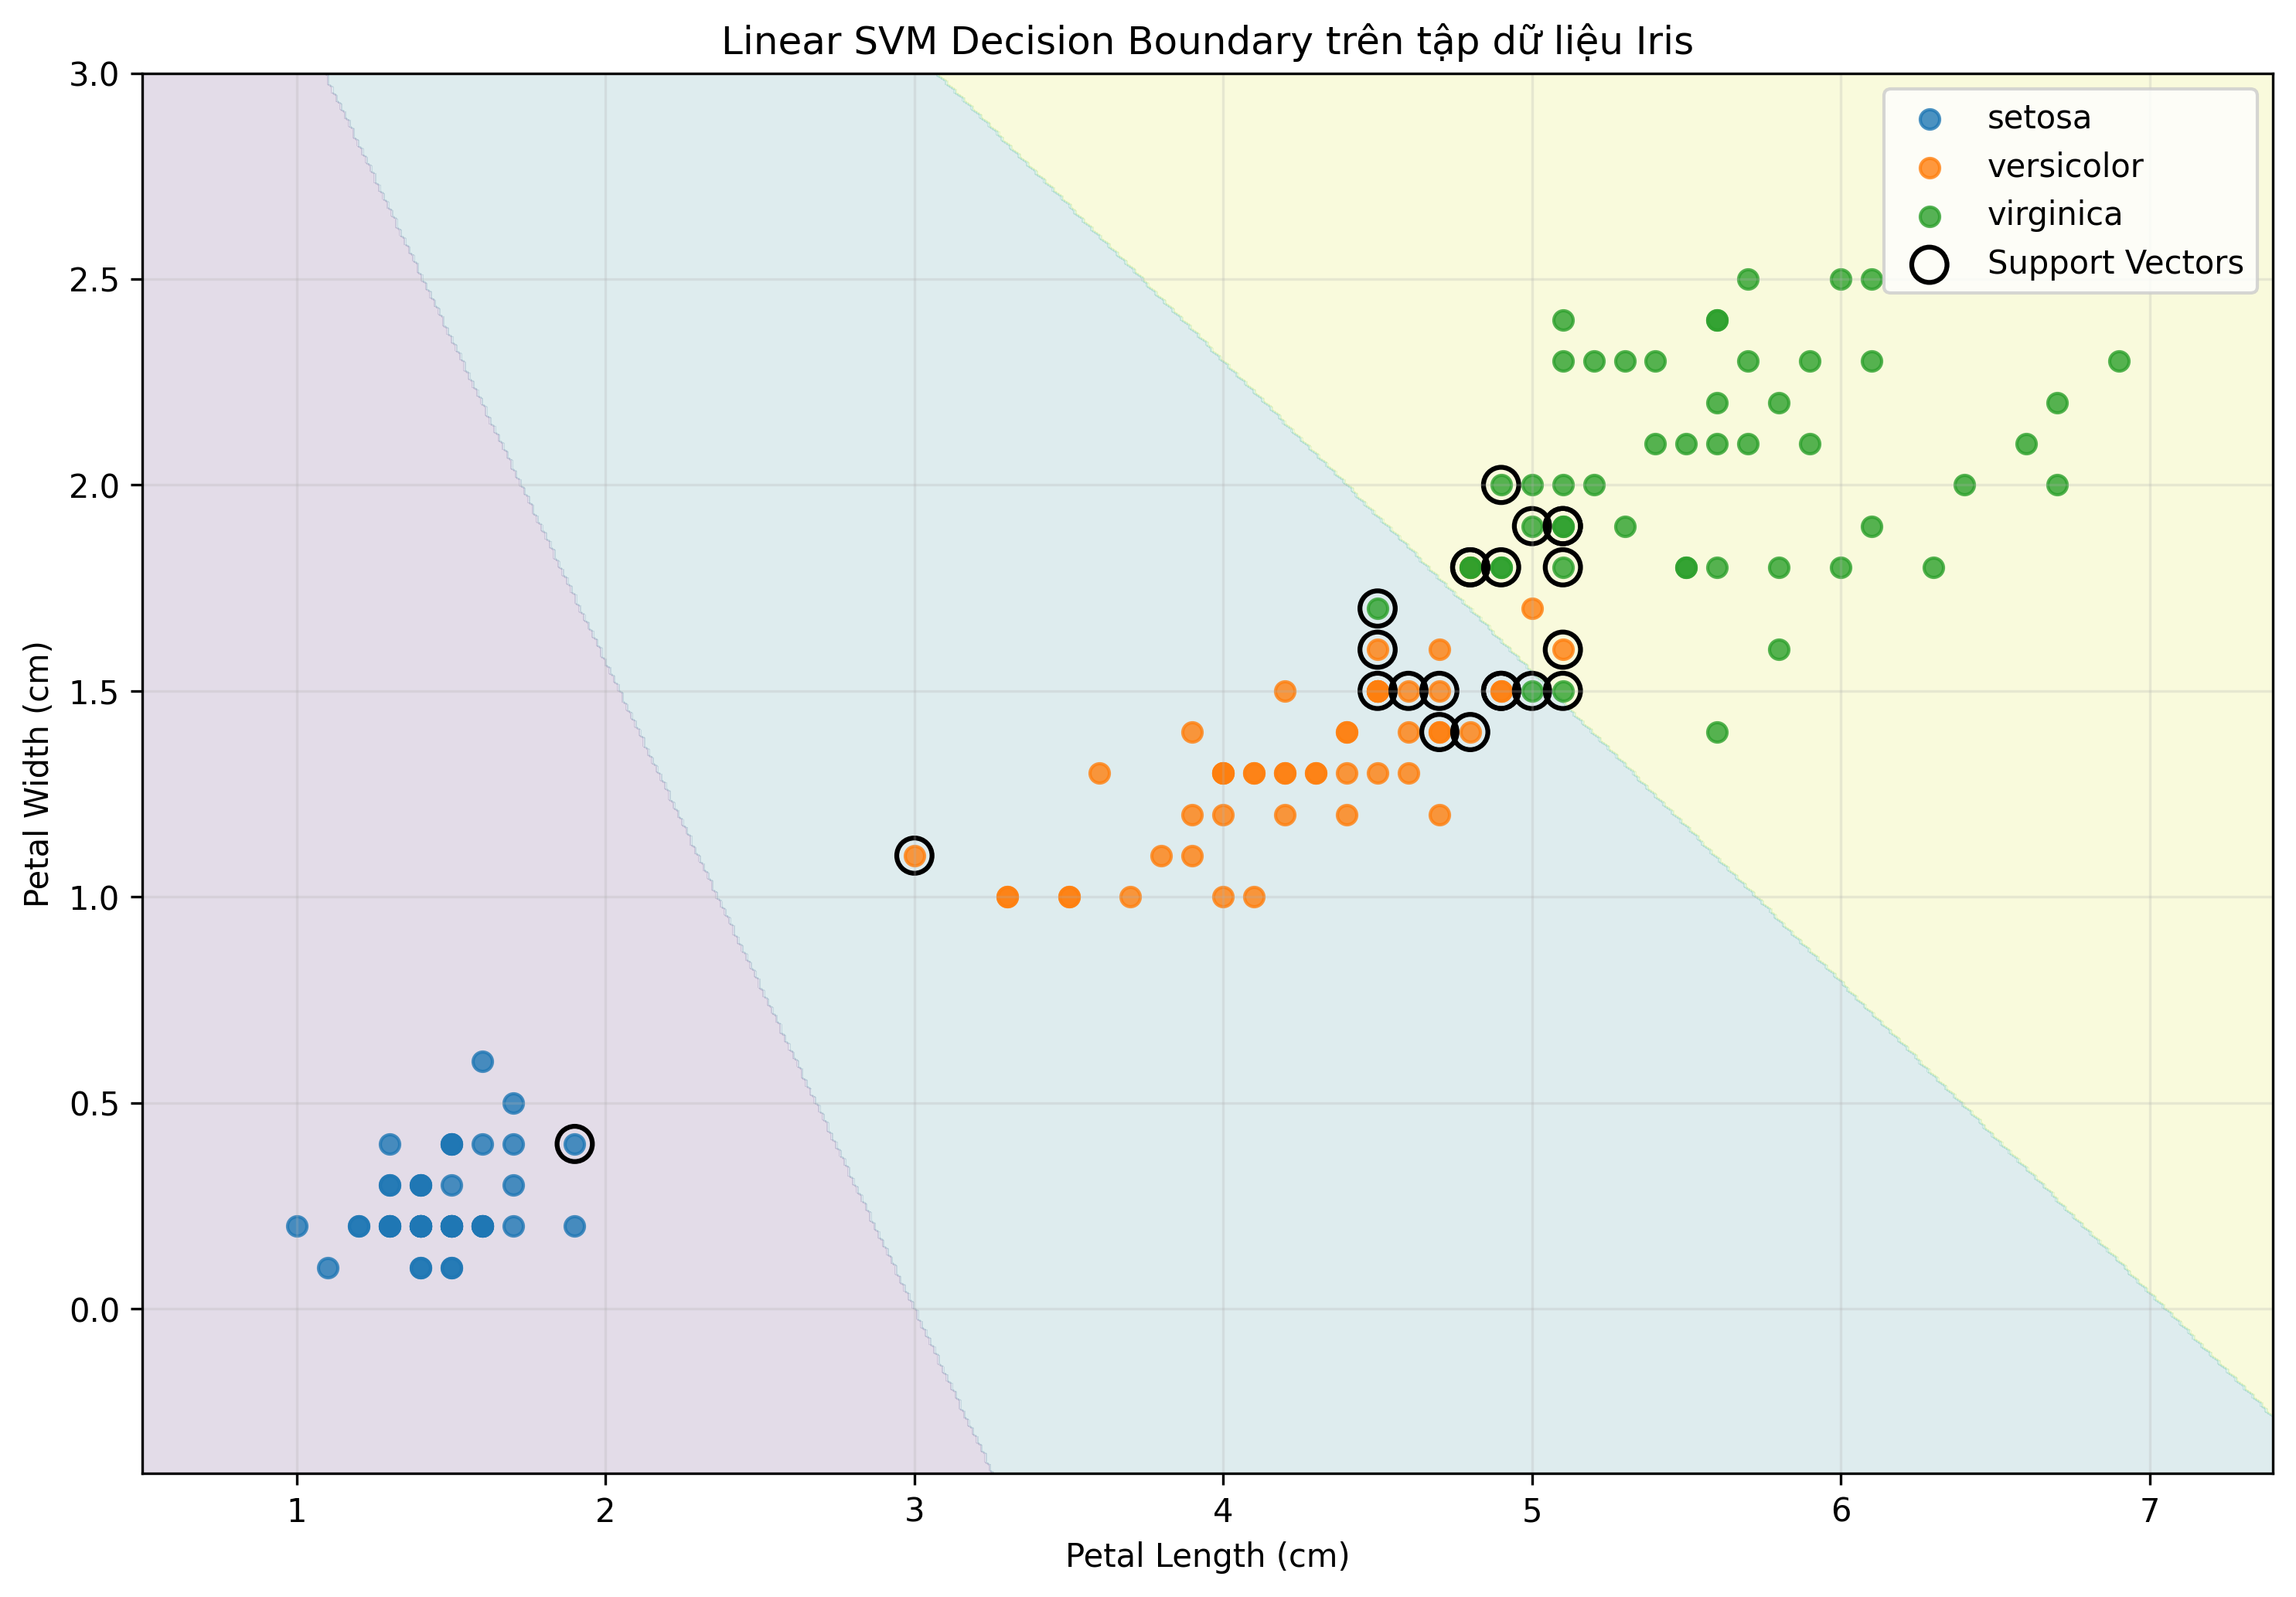
\includegraphics[width=0.9\textwidth]{images/linear_decision_boundary}
	\caption{Đường phân chia tuyến tính của mô hình SVM trên hai đặc trưng Petal Length và Petal Width}
	\label{fig:lineardecisionboundary}
\end{figure}
				\subsection{Các chỉ số đánh giá mô hình}
				
					\noindent Để đánh giá hiệu quả của các mô hình phân loại, đề tài sử dụng các chỉ số Accuracy, Precision, Recall và F1-score.
				
			\subsubsection{Accuracy}
				
					\noindent Accuracy biểu thị tỷ lệ số mẫu được dự đoán đúng trên tổng số mẫu:
				
				\begin{equation*}
					Accuracy =
					\frac{TP+TN}{TP+TN+FP+FN}
				\end{equation*}
				
				Trong đó $TP$, $TN$, $FP$ và $FN$ lần lượt biểu thị số lượng dự đoán
				đúng dương tính, đúng âm tính, sai dương tính và sai âm tính.
				
			\subsubsection{Precision}
				
					\noindent Precision đo lường tỷ lệ các mẫu được mô hình dự đoán là một lớp và thực sự thuộc về lớp đó:
				
				\begin{equation*}
					Precision =
					\frac{TP}{TP+FP}
				\end{equation*}
				
			\subsubsection{Recall}
				
					\noindent Recall biểu thị khả năng mô hình phát hiện đúng các mẫu thực sự thuộc về một lớp:
				
				\begin{equation*}
					Recall =
					\frac{TP}{TP+FN}
				\end{equation*}
				
				\subsubsection{F1-score}
				
				F1-score là trung bình điều hòa giữa Precision và Recall:
				
				\begin{equation*}
					F1 =
					2 \times
					\frac{Precision \times Recall}
					{Precision + Recall}
				\end{equation*}
				
					\noindent Các chỉ số trên được sử dụng để đánh giá và so sánh các mô hình trên cùng tập kiểm thử. Việc sử dụng nhiều chỉ số giúp đánh giá mô hình toàn diện hơn	thay vì chỉ dựa vào Accuracy.\\
					\subsection{Ma trận nhầm lẫn}
					
						\noindent Ma trận nhầm lẫn (Confusion Matrix) là công cụ trực quan hóa kết quả dự đoán của mô hình phân loại. Ma trận cho biết số lượng mẫu thuộc từng lớp thực tế được mô hình dự đoán vào các lớp khác nhau.
					
						\noindent Đối với bài toán Iris gồm ba lớp, ma trận nhầm lẫn có kích thước $3\times3$.Các hàng biểu diễn nhãn thực tế, trong khi các cột biểu diễn nhãn dự đoán.
					
						\noindent Các phần tử trên đường chéo chính thể hiện số mẫu được dự đoán chính xác.
						\noindent Các phần tử nằm ngoài đường chéo thể hiện những trường hợp mô hình dự đoán nhầm giữa các lớp.
					
						\noindent Ma trận nhầm lẫn giúp xác định không chỉ số lượng dự đoán đúng mà còn cho biết mô hình thường nhầm lẫn giữa những lớp nào.
						
	\begin{figure}
		\centering
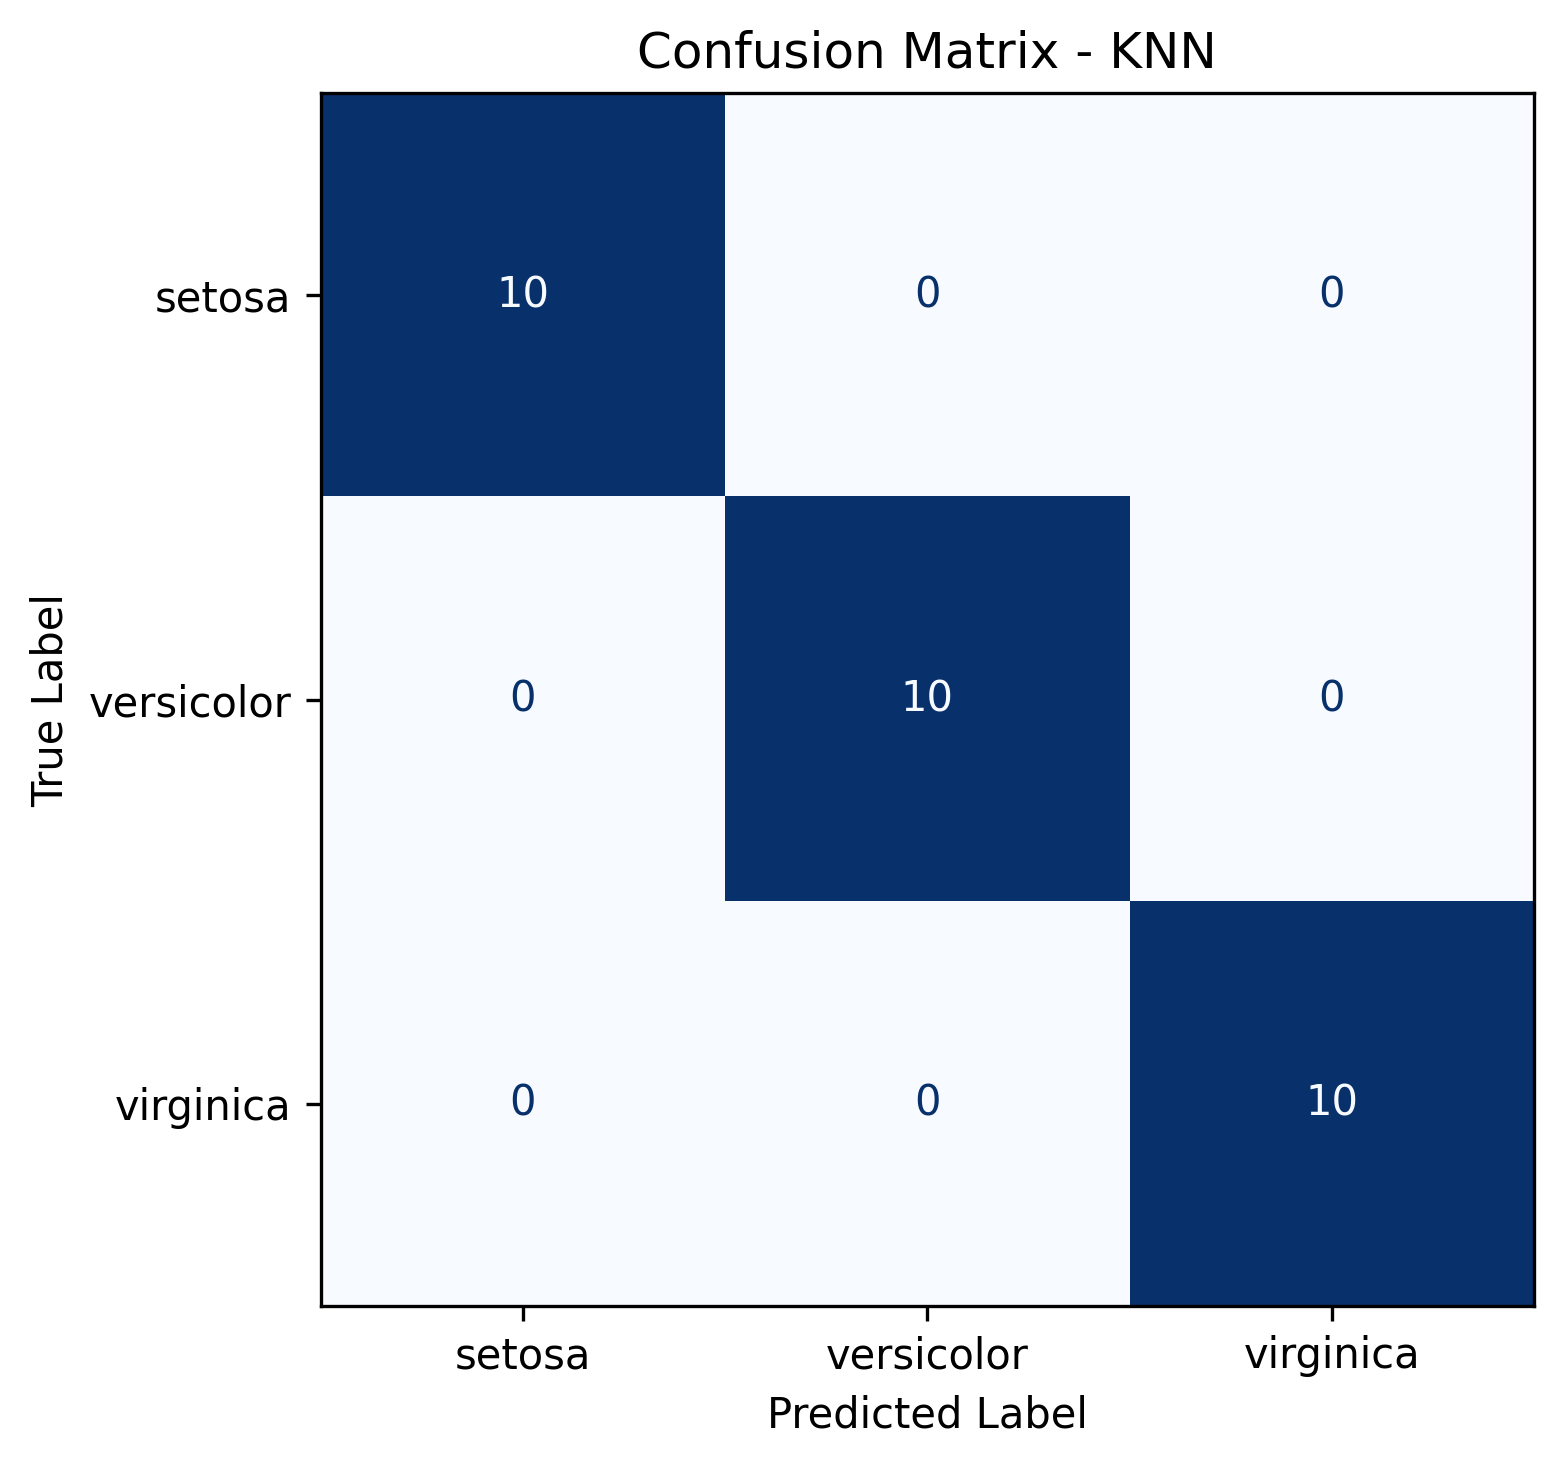
\includegraphics[width=0.3\linewidth]{charts/confusion_matrix_knn}
		 	\hfill
\includegraphics[width=0.30\textwidth]{charts/confusion_matrix_logistic_regression}
		\hfill
			 
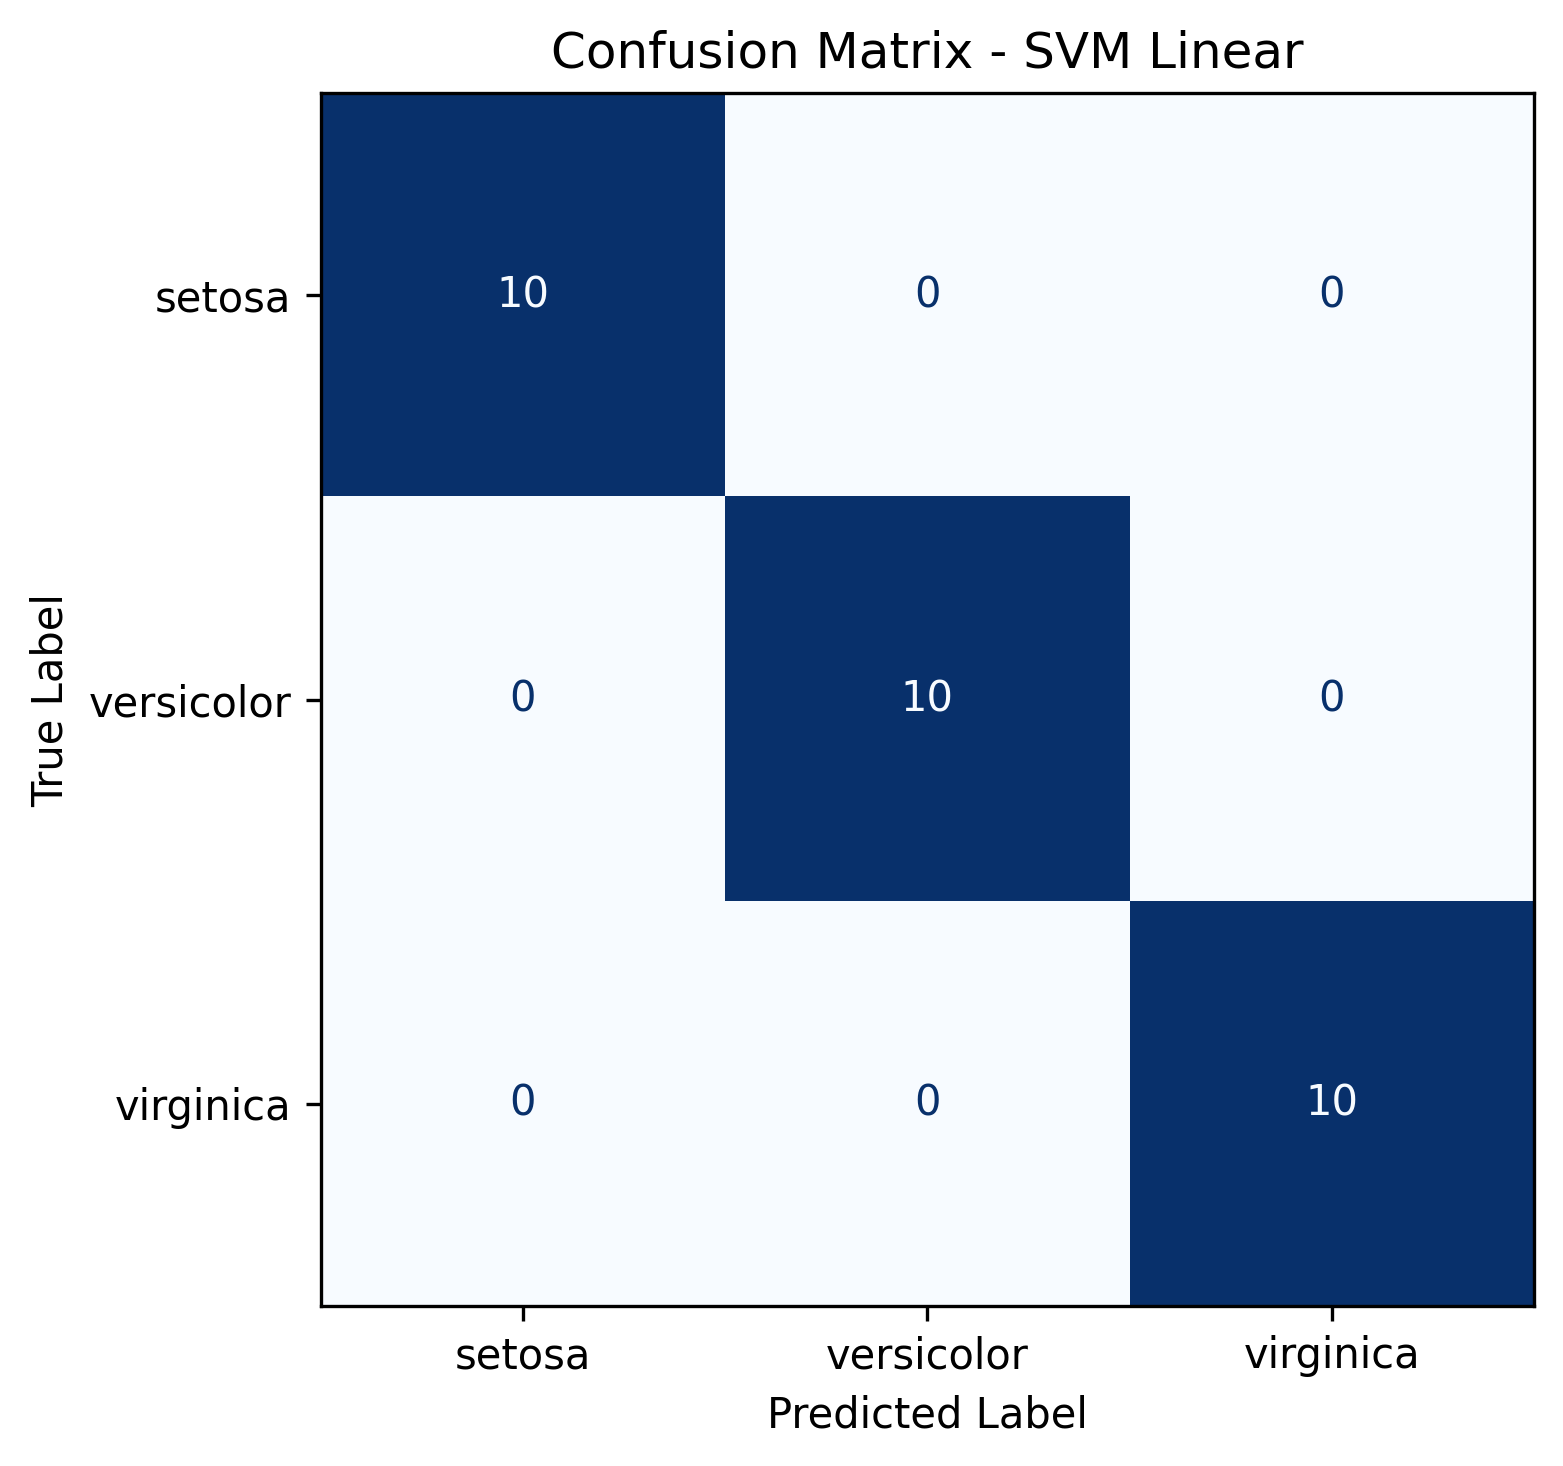
\includegraphics[width=0.30\textwidth]{charts/confusion_matrix_svm_linear}
		\caption{Bộ 3 ma trận nhầm lẫn KNN - LOGISTIC REGRESSION - SVM }
\end{figure}

	
						\subsection{Lưu và triển khai mô hình}
						
						\noindent Sau khi hoàn thành quá trình huấn luyện, mô hình có thể được lưu lại để sử dụng trong ứng dụng mà không cần huấn luyện lại mỗi khi hệ thống khởi động.
						
						\noindent Trong Python, thư viện \texttt{joblib} được sử dụng để lưu mô hình học máy thành tệp. Mô hình sau khi được lưu có thể được tải lại ở phía backend và sử dụng để thực hiện dự đoán trên dữ liệu mới.
						\newpage
						\noindent Quy trình tổng quát gồm:
						
						\begin{enumerate}
							\item Huấn luyện mô hình trên dữ liệu huấn luyện;
							\item Đánh giá mô hình trên tập kiểm thử;
							\item Lưu mô hình đã huấn luyện;
							\item Backend tải mô hình khi ứng dụng khởi động;
							\item API nhận dữ liệu từ người dùng;
							\item Mô hình thực hiện dự đoán;
							\item API trả kết quả về giao diện web.
						\end{enumerate}
						
						\noindent Cách tiếp cận này giúp tách quá trình huấn luyện khỏi quá trình sử dụng mô hình trong ứng dụng thực tế.
						\subsection{API và cơ sở dữ liệu}
						
						\subsubsection{API}
						
							\noindent API (Application Programming Interface) là cơ chế cho phép các thành phần phần mềm trao đổi dữ liệu với nhau thông qua các giao diện được định nghĩa trước.\\
						
							\noindent Trong hệ thống IRIS BOTANICA AI, API được sử dụng để kết nối giao diện web với backend và mô hình học máy. Giao diện gửi dữ liệu đầu vào đến backend,	backend xử lý dữ liệu, thực hiện dự đoán và trả kết quả về cho giao diện.\\
						
							\noindent Bên cạnh API phục vụ mô hình, hệ thống còn xây dựng các chức năng API liên quan đến cơ sở dữ liệu nhằm lưu trữ và truy xuất thông tin người dùng, lịch sử dự đoán và thông tin đánh giá mô hình.\\
						
						\subsubsection{Cơ sở dữ liệu}
						
							\noindent Cơ sở dữ liệu được sử dụng để lưu trữ dữ liệu một cách có tổ chức và cho phép truy xuất khi cần thiết. Trong hệ thống, dữ liệu được tổ chức thành các bảng phục vụ những nhóm thông tin khác nhau.\\
						
						\noindent	Các nhóm dữ liệu chính bao gồm:
						
						\begin{itemize}
							\item Thông tin tài khoản người dùng;
							\item Lịch sử đăng nhập;
							\item Lịch sử dự đoán;
							\item Thông tin mô hình;
							\item Kết quả đánh giá mô hình.
						\end{itemize}
						
						\noindent	Trong quá trình phát triển cục bộ, hệ thống sử dụng SQL Server. Khi triển khai trực tuyến, hệ thống sử dụng PostgreSQL nhằm đáp ứng môi trường cơ sở dữ liệu trên nền tảng Render.\\
						
							\noindent Chi tiết thiết kế cơ sở dữ liệu, cấu trúc  bảng và quá trình kết nối sẽ được trình bày ở các chương tiếp theo.
							
		\newpage 
		
	\section{XÂY DỰNG VÀ TRIỂN KHAI HỆ THỐNG IRIS BOTANICA AI}
	
	\subsection{Kiến trúc tổng thể của hệ thống}
	
	\noindent Sau khi hoàn thành quá trình khảo sát dữ liệu, huấn luyện và đánh giá mô hình SVM, bước tiếp theo của đề tài là đóng gói mô hình thành một hệ thống có khả năng tương tác trực tiếp với người dùng thông qua môi trường Web. Sản phẩm cuối cùng được xây dựng với tên gọi \textbf{IRIS BOTANICA AI}, có nhiệm vụ tiếp nhận các thông số hình thái của một mẫu hoa Iris, sử dụng mô hình SVM đã huấn luyện để thực hiện dự đoán và trả kết quả trực quan cho người dùng.
	
	\noindent Hệ thống được xây dựng theo kiến trúc gồm nhiều thành phần liên kết với nhau. Trong đó, giao diện Web đảm nhận nhiệm vụ tương tác với người dùng; FastAPI đóng vai trò là lớp Backend trung gian; mô hình SVM thực hiện nhiệm vụ phân loại; API CSDL đảm nhận việc trao đổi dữ liệu với cơ sở dữ liệu; hệ thống người dùng quản lý tài khoản và phiên đăng nhập; cơ sở dữ liệu lưu trữ thông tin tài khoản, lịch sử dự đoán và các thông tin liên quan đến quá trình vận hành.
	
\begin{figure}[tbph]
	\centering
	\includegraphics[width=0.95\textwidth]{"images/ảnh kiến trúc"}
	\caption{Kiến trúc tổng thể của hệ thống IRIS BOTANICA AI}
	\label{fig:anh-kien-truc}
\end{figure}
	

	
	\noindent Luồng xử lý tổng quát của hệ thống được thực hiện theo trình tự:
	
	\begin{enumerate}[leftmargin=*]
		\item Người dùng truy cập giao diện Web IRIS BOTANICA AI.
		\item Người dùng đăng ký hoặc đăng nhập tài khoản.
		\item Người dùng nhập bốn thông số hình thái của mẫu hoa Iris.
		\item Frontend gửi dữ liệu đến Backend thông qua API.
		\item FastAPI kiểm tra dữ liệu đầu vào và chuyển dữ liệu về đúng cấu trúc mà mô hình SVM yêu cầu.
		\item Mô hình SVM được nạp từ tập tin \texttt{svm model.pkl} và thực hiện dự đoán.
		\item Kết quả dự đoán được trả về cho giao diện Web.
		\item Hệ thống ghi nhận thời gian thực hiện dự đoán và lưu kết quả vào cơ sở dữ liệu.
		\item Người dùng có thể xem lại lịch sử dự đoán của mình trên giao diện Web.
	\end{enumerate}
	
	\subsection{Chuẩn bị môi trường và cấu trúc dự án}
				    \vspace{-0.3cm}
	\noindent Hệ thống được phát triển bằng ngôn ngữ Python. Môi trường lập trình được xây dựng nhằm phục vụ đồng thời ba nhóm nhiệm vụ: huấn luyện mô hình học máy, xây dựng Backend API và kết nối với cơ sở dữ liệu.
	
	\noindent Các công nghệ chính được sử dụng trong đề tài gồm:
	
	\begin{itemize}[leftmargin=*]
		\item \textbf{Python:} ngôn ngữ lập trình chính dùng để huấn luyện mô hình và xây dựng Backend.
		\item \textbf{Scikit-learn:} thư viện cung cấp thuật toán Support Vector Machine và các công cụ đánh giá mô hình.
		\item \textbf{Joblib:} thư viện dùng để lưu và nạp mô hình học máy.
		\item \textbf{FastAPI:} framework dùng để xây dựng các Web API.
		\item \textbf{Pydantic:} hỗ trợ kiểm tra và xác thực dữ liệu đầu vào cho API.
		\item \textbf{NumPy:} hỗ trợ chuyển đổi dữ liệu đầu vào thành cấu trúc mảng phù hợp với mô hình.
		\item \textbf{SQLAlchemy:} hỗ trợ kết nối và thực hiện các thao tác với cơ sở dữ liệu.
		\item \textbf{SQLite:} cơ sở dữ liệu được sử dụng để lưu trữ thông tin của hệ thống.
		\item \textbf{HTML, CSS và JavaScript:} xây dựng giao diện và xử lý tương tác phía người dùng.
		\item \textbf{Uvicorn:} máy chủ ASGI dùng để chạy ứng dụng FastAPI.
		\item \textbf{Render:} nền tảng triển khai ứng dụng trực tuyến.
	\end{itemize}
	
	\noindent Cấu trúc dự án được tổ chức thành các thành phần riêng biệt nhằm thuận tiện cho việc phát triển và bảo trì hệ thống. Các thành phần quan trọng gồm tập tin huấn luyện mô hình, tập tin mô hình đã lưu, mã nguồn FastAPI, các thành phần kết nối cơ sở dữ liệu và giao diện Web.
	
	
	
	\subsection{Huấn luyện và đánh giá mô hình SVM}
	
	\noindent Quá trình huấn luyện mô hình SVM đã được trình bày chi tiết ở Chương 2. Trong Chương 3, kết quả của quá trình này được sử dụng làm đầu vào cho giai đoạn triển khai hệ thống.
	
	\noindent Mô hình được xây dựng bằng lớp \texttt{SVC} của thư viện Scikit-learn với lựa chọn:
	
	\begin{lstlisting}[language=Python, numbers=none]
		model = SVC(kernel="linear")
	\end{lstlisting}
	
	\noindent Dữ liệu được chia thành tập huấn luyện và tập kiểm thử theo tỷ lệ 80/20, đồng thời sử dụng \texttt{stratify=y} để duy trì tỷ lệ các lớp. Kết quả kiểm thử của mô hình trên 30 mẫu thuộc tập Test đạt độ chính xác 100\% theo thực nghiệm của đề tài.
	
	\noindent Cần phân biệt rõ hai giai đoạn. Tập Test được sử dụng để đánh giá khả năng tổng quát hóa của mô hình, trong khi sau khi hoàn thành đánh giá, mô hình được huấn luyện lại trên toàn bộ 150 mẫu để tạo phiên bản cuối cùng phục vụ triển khai Web.
	
	\subsection{Xây dựng đường phân chia tuyến tính}
	
	\noindent Một trong những nội dung quan trọng của đề tài là trực quan hóa đường phân chia do mô hình SVM tạo ra. Với SVM sử dụng Kernel tuyến tính, ranh giới quyết định được biểu diễn dưới dạng một siêu phẳng:
	
	$$
	w^T x+b=0
	$$
	
	\noindent Trong đó, $x$ là vector đặc trưng của một mẫu dữ liệu, $w$ là vector trọng số và $b$ là hệ số dịch. Với dữ liệu hai chiều, phương trình trên tương ứng với một đường thẳng. Đối với dữ liệu Iris có bốn đặc trưng, ranh giới phân loại thực tế tồn tại trong không gian bốn chiều và có thể được gọi là siêu phẳng phân chia.\\
	
	\noindent Do không gian dữ liệu Iris có bốn chiều nên không thể biểu diễn trực tiếp toàn bộ siêu phẳng trên một mặt phẳng hai chiều. Vì vậy, đề tài sử dụng các cặp đặc trưng tiêu biểu để trực quan hóa xu hướng phân tách của các lớp dữ liệu.\\
	
	\noindent Đặc biệt, hai đặc trưng \text{petal length} và \text{petal width} thể hiện khả năng phân biệt rõ giữa các loài Iris. Việc trực quan hóa giúp minh họa trực quan nguyên lý hoạt động của SVM: tìm ranh giới có khả năng phân tách các nhóm dữ liệu với khoảng cách lề phù hợp.
	
\begin{figure}[tbph]
	\centering
	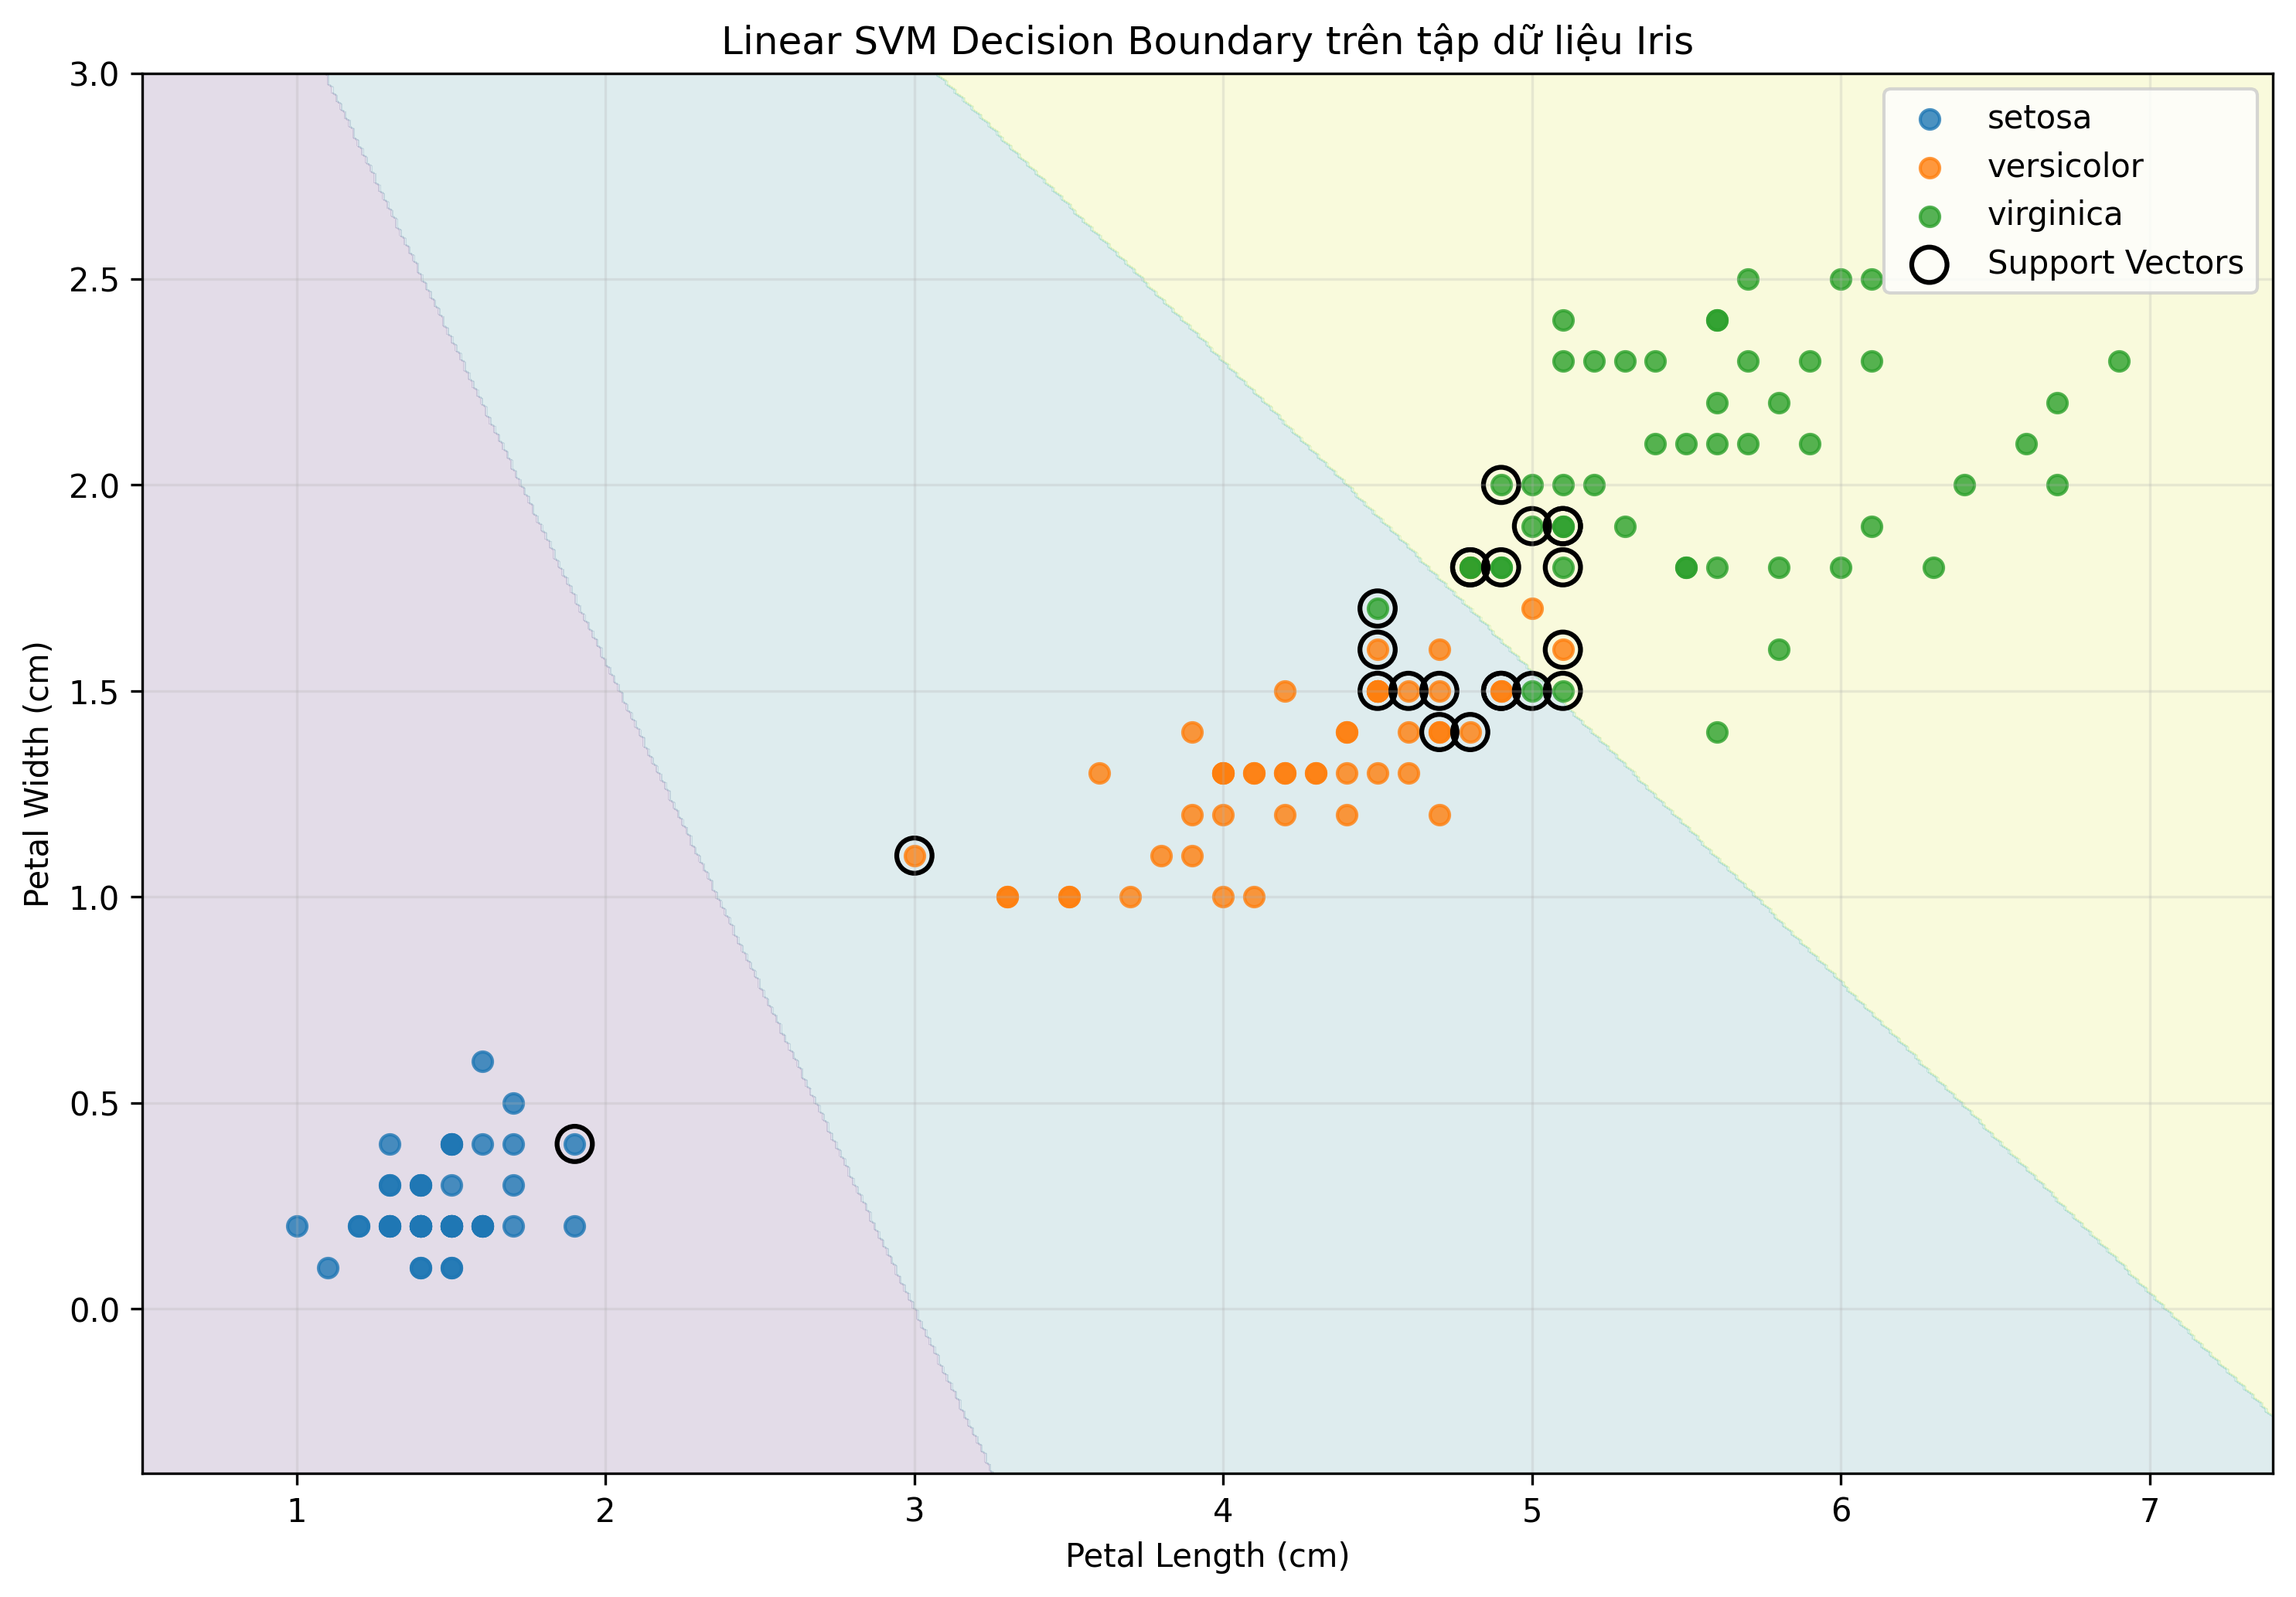
\includegraphics[width=0.7\textwidth]{images/linear_decision_boundary}
	\caption{Trực quan hóa đường phân chia tuyến tính trên dữ liệu Iris}
	\label{fig:lineardecisionboundary}
\end{figure}
	

	\noindent Đường phân chia tuyến tính không phải là một bước huấn luyện riêng biệt sau khi mô hình đã được lưu. Đây là cách trực quan hóa và phân tích ranh giới quyết định được hình thành từ quá trình huấn luyện SVM. Do đó, quy trình hợp lý là: dữ liệu được sử dụng để huấn luyện mô hình, mô hình tạo ra các tham số phân loại, sau đó các tham số này được sử dụng để trực quan hóa đường phân chia và cuối cùng mô hình được lưu để triển khai.
	
	\subsection{Lưu và sử dụng mô hình}
	
	\noindent Sau khi đánh giá mô hình, phiên bản cuối cùng được huấn luyện trên toàn bộ tập dữ liệu Iris gồm 150 mẫu. Mô hình sau khi huấn luyện được lưu dưới dạng tập tin nhị phân \text{svm model.pkl} bằng thư viện Joblib.
	
	\begin{lstlisting}[language=Python, numbers=none]
		final_model = SVC(kernel="linear")
		final_model.fit(X, y)
		
		joblib.dump(final_model, "svm_model.pkl")
	\end{lstlisting}
	
	\noindent Việc lưu mô hình giúp tách biệt quá trình huấn luyện và quá trình dự đoán. Khi triển khai Web, hệ thống không cần huấn luyện lại mô hình mỗi khi có người dùng gửi yêu cầu. Backend chỉ cần nạp mô hình đã được huấn luyện bằng:
	
	\begin{lstlisting}[language=Python, numbers=none]
		model = joblib.load("svm_model.pkl")
	\end{lstlisting}
	
	\noindent Nhờ đó, quá trình dự đoán trên Web được thực hiện nhanh chóng và tránh lặp lại quá trình huấn luyện không cần thiết.\\
	
	
	\noindent
	Sau khi khởi động hệ thống FastAPI, mô hình SVM được nạp tự động từ tệp
	\text{svm\_model.pkl} thông qua thư viện \texttt{joblib}. 
	Quá trình này được thực hiện thành công trước khi hệ thống tiếp nhận các yêu cầu dự đoán từ người dùng.
	\begin{lstlisting}[language=Python, caption={Nạp mô hình SVM khi khởi động hệ thống}]
		model = joblib.load("svm_model.pkl")
		print("Model svm_model.pkl loaded successfully!")
	\end{lstlisting}
	
	\subsection{Xây dựng API mô hình bằng FastAPI}
	
	\noindent Sau khi có mô hình đã lưu, FastAPI được sử dụng để xây dựng lớp API trung gian giữa giao diện Web và mô hình SVM. API có nhiệm vụ tiếp nhận dữ liệu, kiểm tra dữ liệu, gọi mô hình dự đoán và trả kết quả dưới dạng JSON.
	
	\subsubsection{Khởi tạo ứng dụng FastAPI}
	
	\noindent Ứng dụng được khởi tạo bằng lớp \text{FastAPI}. Mô hình SVM được nạp khi Backend khởi động để sẵn sàng phục vụ các yêu cầu dự đoán.
	
	\begin{lstlisting}[language=Python, numbers=none]
		app = FastAPI(
		title="Iris Flower Classification API",
		description="API for Iris flower classification using SVM model",
		version="1.0.0"
		)
		
		model = joblib.load("svm_model.pkl")
	\end{lstlisting}
	
	\subsubsection{Xây dựng API dự đoán}
	
	\noindent Endpoint \text{/predict} tiếp nhận bốn thông số gồm chiều dài đài hoa, chiều rộng đài hoa, chiều dài cánh hoa và chiều rộng cánh hoa.
	\newpage
	\begin{lstlisting}[language=Python, numbers=none]
		@app.post("/predict")
		def predict_iris(data: IrisInput):
		
		
		input_features = np.array([[
		data.sepal_length,
		data.sepal_width,
		data.petal_length,
		data.petal_width
		]])
		
		prediction_id = int(model.predict(input_features)[0])
		predicted_class = CLASS_NAMES[prediction_id]
		
		return {
			"input": {
				"sepal_length": data.sepal_length,
				"sepal_width": data.sepal_width,
				"petal_length": data.petal_length,
				"petal_width": data.petal_width
			},
			"prediction_id": prediction_id,
			"predicted_class": predicted_class
		}
	
		
	\end{lstlisting}
	
	\noindent Dữ liệu đầu vào được chuyển thành mảng NumPy có kích thước $1\times4$, phù hợp với cấu trúc dữ liệu mà mô hình Scikit-learn yêu cầu.
	
	\subsubsection{Kiểm tra dữ liệu đầu vào}
	
	\noindent Pydantic được sử dụng để định nghĩa cấu trúc dữ liệu đầu vào. Các trường dữ liệu được khai báo dưới dạng số thực và yêu cầu giá trị lớn hơn 0.
	
	\begin{lstlisting}[language=Python, numbers=none]
		class IrisInput(BaseModel):
		sepal_length: float = Field(..., gt=0)
		sepal_width: float = Field(..., gt=0)
		petal_length: float = Field(..., gt=0)
		petal_width: float = Field(..., gt=0)
	\end{lstlisting}
	
	\noindent Cơ chế này giúp hạn chế dữ liệu không hợp lệ trước khi dữ liệu được chuyển tới mô hình học máy.
	
\begin{figure}[tbph]
	\centering
	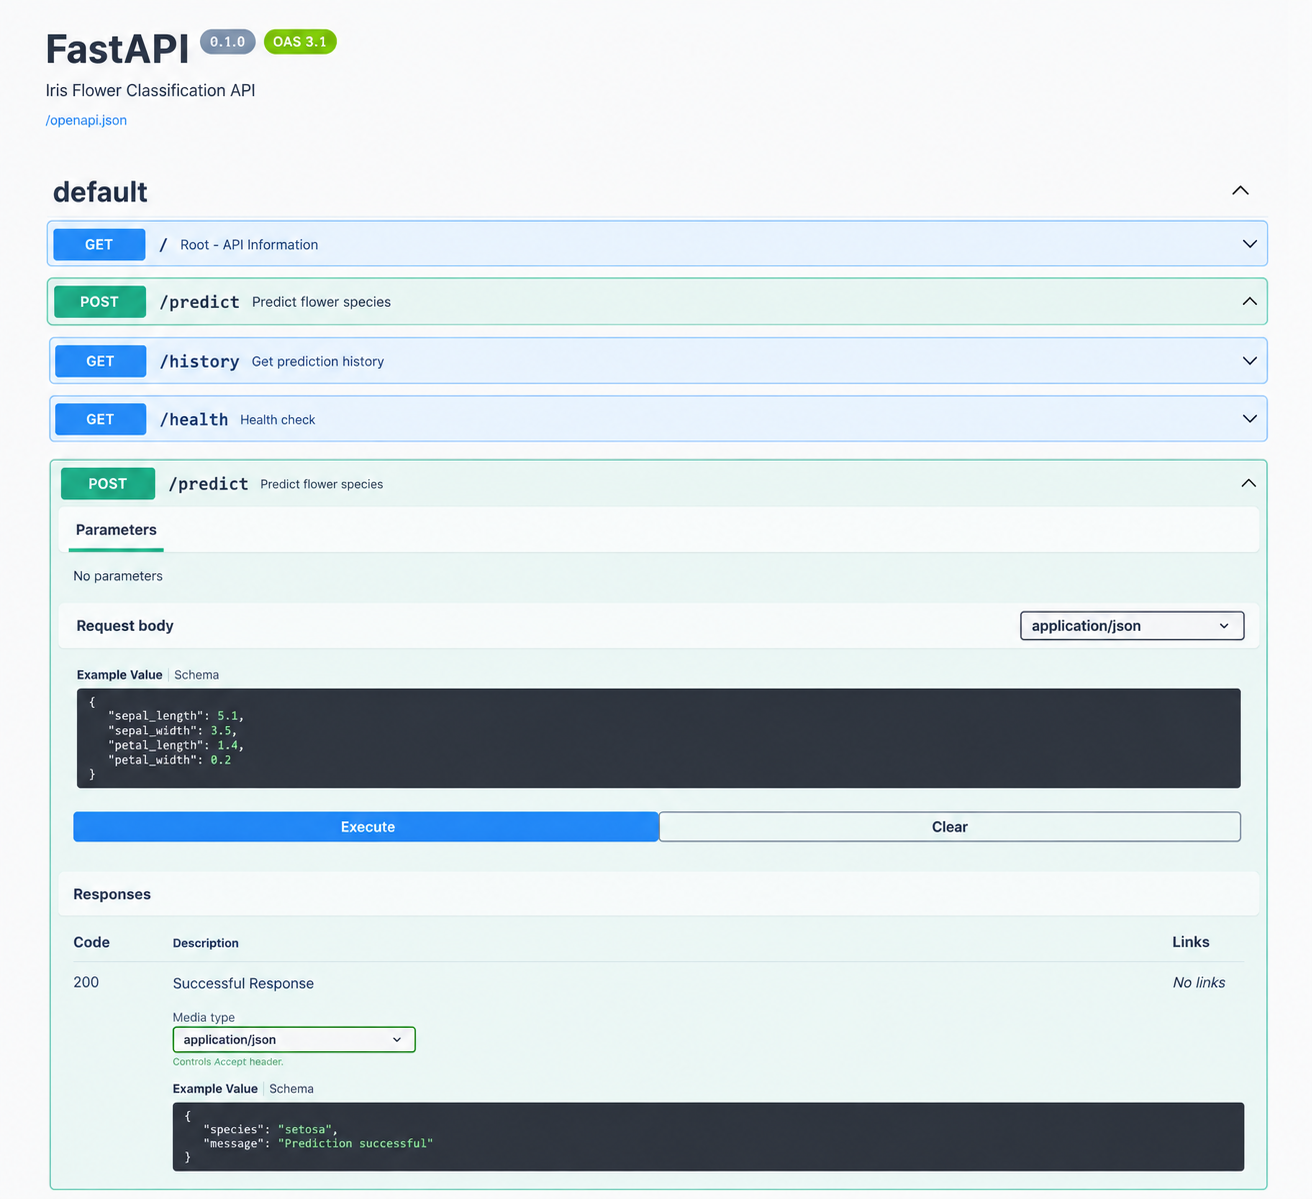
\includegraphics[width=0.5\textwidth]{images/api_predict.png}
	\caption{API dự đoán hoa Iris trên Swagger UI}
	\label{fig:apipredict}
\end{figure}
	
	
	\subsection{Xây dựng API CSDL}
	
	\noindent Bên cạnh API phục vụ dự đoán, hệ thống còn xây dựng lớp API phục vụ trao đổi dữ liệu với cơ sở dữ liệu. Việc tách riêng chức năng này giúp Backend quản lý rõ ràng hai nhóm nhiệm vụ: xử lý mô hình học máy và xử lý dữ liệu hệ thống.
	
	\noindent API CSDL được sử dụng để thực hiện các thao tác như tạo tài khoản, kiểm tra thông tin đăng nhập, lưu lịch sử dự đoán và truy vấn lịch sử của người dùng.
	
	\noindent Quy trình trao đổi dữ liệu có thể khái quát:
	
	$$
	\text{Web} \rightarrow \text{API} \rightarrow \text{Database Layer} \rightarrow \text{SQLite}
	$$
	
	\noindent Khi người dùng thực hiện một thao tác yêu cầu lưu hoặc truy xuất dữ liệu, Frontend gửi yêu cầu đến Backend. Backend tiếp nhận yêu cầu, thực hiện kiểm tra và sử dụng lớp kết nối CSDL để thực hiện câu lệnh tương ứng.
	
	\begin{figure}[htbp]
		\centering
		
		\begin{tikzpicture}[
			node distance=1.8cm,
			box/.style={
				draw,
				rounded corners=2pt,
				minimum width=5.5cm,
				minimum height=0.9cm,
				align=center,
				font=\small
			}
			]
			
			\node[box] (web) {Web Iris Botanica AI};
			
			\node[box, below=1.8cm of web] (api)
			{FastAPI Backend\\API xử lý dữ liệu};
			
			\node[box, below=1.8cm of api] (dbapi)
			{Database API\\Kết nối và truy vấn};
			
			\node[box, below=1.8cm of dbapi] (database)
			{SQLite Database\\Người dùng -- Lịch sử -- Dự đoán};
			
			\draw[->, thick] (web) -- (api);
			\draw[->, thick] (api) -- (dbapi);
			\draw[->, thick] (dbapi) -- (database);
			
		\end{tikzpicture}
		
		\caption{Kiến trúc kết nối giữa Web, API và cơ sở dữ liệu}

	\end{figure}
	
	
	\subsection{Xây dựng hệ thống người dùng}
	
	\noindent Để hệ thống có khả năng phân biệt dữ liệu của từng người sử dụng, đề tài bổ sung cơ chế quản lý tài khoản. Người dùng có thể tạo tài khoản, đăng nhập và sử dụng các chức năng dự đoán trên hệ thống.
	
	\subsubsection{Đăng ký tài khoản}
	
	\noindent Khi người dùng đăng ký, hệ thống tiếp nhận tên đăng nhập và mật khẩu. Backend kiểm tra thông tin trước khi lưu vào cơ sở dữ liệu. Nếu tên đăng nhập đã tồn tại, hệ thống trả về thông báo tương ứng thay vì tạo bản ghi trùng lặp.
	
	\noindent Việc lưu tài khoản vào CSDL giúp thông tin người dùng được duy trì giữa các lần sử dụng ứng dụng.
	
\begin{figure}[tbph]
	\centering
	\includegraphics[width=0.65\textwidth]{"images/đăng ký"}
	\caption{Giao diện đăng ký tài khoản, yêu cầu 8 chữ số}
	\label{fig:ang-ky}
\end{figure}
	
	
	
	\subsubsection{Đăng nhập}
	
	\noindent Sau khi có tài khoản, người dùng có thể đăng nhập bằng tên đăng nhập và mật khẩu. Backend kiểm tra thông tin với dữ liệu được lưu trong cơ sở dữ liệu. Nếu thông tin chính xác, hệ thống tạo trạng thái đăng nhập cho người dùng.
	
\begin{figure}[tbph]
	\centering
	\includegraphics[width=0.65\textwidth]{"images/đăng nhập"}
	\caption{Giao diện đăng nhập hệ thống}
	\label{fig:ang-nhap}
\end{figure}
	
	
	\subsubsection{Quản lý phiên đăng nhập}
	
	\noindent Sau khi đăng nhập thành công, hệ thống cần duy trì trạng thái người dùng trong phiên làm việc. Cơ chế phiên giúp Backend xác định người dùng hiện tại khi người dùng thực hiện các thao tác tiếp theo như dự đoán hoặc xem lịch sử.
	
	\noindent Việc quản lý phiên cũng giúp hệ thống gắn kết dữ liệu lịch sử dự đoán với đúng tài khoản đang sử dụng, thay vì lưu dữ liệu một cách không phân biệt.
	
	\subsection{Xây dựng chức năng lưu trữ lịch sử dự đoán}
	
	\noindent Một trong những chức năng mở rộng của hệ thống là lưu lại các lần dự đoán. Mỗi khi người dùng thực hiện dự đoán, hệ thống có thể ghi nhận thông tin đầu vào, kết quả dự đoán, tài khoản thực hiện và thời gian xử lý.
	
	\subsubsection{Lưu kết quả dự đoán}
	
	\noindent Sau khi mô hình SVM trả về kết quả, Backend thực hiện quá trình lưu dữ liệu vào cơ sở dữ liệu. Việc lưu trữ được thực hiện sau khi quá trình dự đoán hoàn thành để đảm bảo dữ liệu lịch sử phản ánh đúng kết quả mà hệ thống đã trả về.
	
	\noindent Thông tin lịch sử có thể bao gồm:
	
	\begin{itemize}[leftmargin=*]
		\item Tài khoản thực hiện dự đoán.
		\item Bốn thông số đầu vào của mẫu hoa.
		\item Loài hoa được dự đoán.
		\item Mã mô hình được sử dụng.
		\item Thời gian thực hiện dự đoán.
		\item Thời gian chạy mô hình.
		\item Trạng thái bản ghi.
	\end{itemize}
	
	\subsubsection{Xem lịch sử dự đoán}
	
	\noindent Người dùng sau khi đăng nhập có thể truy cập chức năng lịch sử để xem lại các lần dự đoán trước đó. Dữ liệu được truy vấn dựa trên tài khoản đang đăng nhập, giúp mỗi người dùng chỉ xem được dữ liệu thuộc phạm vi được hệ thống cho phép.
	
\begin{figure}[tbph]
	\centering
	\includegraphics[width=0.90\textwidth]{"images/lịch sử dự đoán"}
	\caption{Giao diện hiển thị lịch sử dự đoán}
	\label{fig:lich-su-du-oan}
\end{figure}
	
	
	\subsubsection{Xóa mềm và khôi phục dữ liệu}
	
	\noindent Đối với những bản ghi lịch sử không còn cần hiển thị, hệ thống có thể sử dụng cơ chế xóa mềm. Thay vì xóa ngay dữ liệu khỏi cơ sở dữ liệu, bản ghi được chuyển sang trạng thái không hoạt động.
	
	\noindent Cách tiếp cận này giúp hạn chế mất dữ liệu ngoài ý muốn và tạo khả năng khôi phục bản ghi khi cần thiết.
	
	\subsubsection{Xóa vĩnh viễn}
	
	\noindent Trong trường hợp người dùng hoặc hệ thống xác định một bản ghi không còn cần thiết, dữ liệu có thể được xóa vĩnh viễn khỏi cơ sở dữ liệu. Chức năng này được tách biệt với xóa mềm nhằm tránh việc xóa dữ liệu ngoài ý muốn trong thao tác thông thường.
	
	\subsection{Ghi nhận thời gian chạy mô hình}
	
	\noindent Ngoài kết quả dự đoán, hệ thống còn ghi nhận thời gian thực hiện mô hình nhằm phục vụ đánh giá hiệu năng của quá trình suy luận.
	
	\noindent Quy trình đo thời gian được thực hiện theo nguyên tắc:
	
	$$
	T_{\text{chạy}} =
	T_{\text{kết thúc}} -
	T_{\text{bắt đầu}}
	$$
	
	\noindent Trong đó thời điểm bắt đầu được ghi nhận trước khi gọi hàm dự đoán và thời điểm kết thúc được ghi nhận sau khi mô hình trả về kết quả.
	
	\begin{lstlisting}[language=Python, numbers=none]
		import time
		
		start_time = time.perf_counter()
		
		prediction_id = int(model.predict(input_features)[0])
		
		end_time = time.perf_counter()
		
		runtime = end_time - start_time
	\end{lstlisting}
	
	\noindent Thông tin thời gian chạy có thể được lưu cùng kết quả dự đoán để phục vụ quá trình theo dõi hiệu năng hệ thống.
	
	\noindent Trong báo cáo, thời gian chạy cần được trình bày dựa trên kết quả đo thực tế của hệ thống thay vì sử dụng một giá trị cố định không có nguồn đo.
	
	\subsection{Kết nối hệ thống với cơ sở dữ liệu}
	
	\noindent Cơ sở dữ liệu đóng vai trò lưu trữ dữ liệu phát sinh trong quá trình vận hành hệ thống. Trong phạm vi đề tài, SQLite được sử dụng do có cấu trúc đơn giản, không yêu cầu triển khai một máy chủ CSDL riêng và phù hợp với quy mô dữ liệu của ứng dụng.
	
	\noindent Lớp kết nối được tổ chức riêng nhằm giúp các module khác của hệ thống có thể sử dụng lại kết nối CSDL mà không phải viết lại toàn bộ logic kết nối.
	
	\noindent Kiến trúc xử lý dữ liệu có thể mô tả:
	
\begin{figure}[htbp]
	\centering
	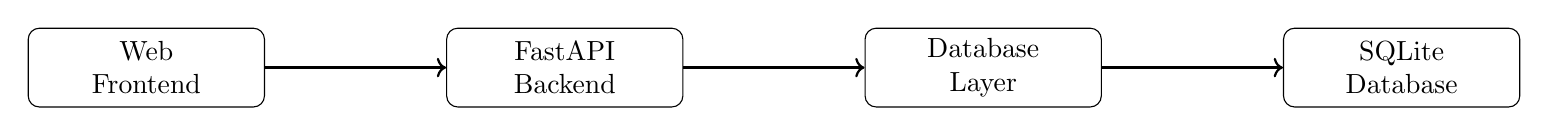
\begin{tikzpicture}[
		node distance=1.3cm,
		box/.style={
			draw,
			rounded corners,
			minimum width=3cm,
			minimum height=1cm,
			align=center
		}
		]
		
		\node (web) [box] {Web\\Frontend};
		
		\node (api) [box, right=of web, xshift=1cm]
		{FastAPI\\Backend};
		
		\node (dbapi) [box, right=of api, xshift=1cm]
		{Database\\Layer};
		
		\node (db) [box, right=of dbapi, xshift=1cm]
		{SQLite\\Database};
		
		\draw[->, thick] (web) -- (api);
		\draw[->, thick] (api) -- (dbapi);
		\draw[->, thick] (dbapi) -- (db);
		
	\end{tikzpicture}
	\caption{Luồng kết nối giữa Web, Backend và cơ sở dữ liệu}
	\label{fig:database-flow}
\end{figure}


	
	\noindent Sự phân tách này giúp hệ thống có cấu trúc rõ ràng hơn và thuận tiện khi mở rộng sang hệ quản trị cơ sở dữ liệu khác trong tương lai.
	
	\subsection{Xây dựng giao diện Web IRIS BOTANICA AI}
	
	\noindent Giao diện Web là lớp tương tác trực tiếp với người dùng. Thiết kế của hệ thống hướng đến việc đơn giản hóa thao tác: người dùng không cần biết cách mô hình SVM hoạt động bên trong mà chỉ cần cung cấp các thông số của mẫu hoa.
	
	\noindent Giao diện chính cung cấp các khu vực nhập bốn thông số:
	
	\begin{itemize}[leftmargin=*]
		\item Chiều dài đài hoa.
		\item Chiều rộng đài hoa.
		\item Chiều dài cánh hoa.
		\item Chiều rộng cánh hoa.
	\end{itemize}
	
	\noindent Sau khi người dùng thực hiện dự đoán, giao diện nhận phản hồi từ API và hiển thị tên loài hoa tương ứng.
	
\begin{figure}[tbph]
	\centering
	\includegraphics[width=0.92\textwidth]{"images/web chính"}
	\caption{Giao diện chính của hệ thống IRIS BOTANICA AI}
	\label{fig:web-chinh}
\end{figure}
	
	\noindent Giao diện Web được xây dựng bằng HTML, CSS và JavaScript. JavaScript đảm nhận việc lấy dữ liệu từ biểu mẫu, gửi yêu cầu đến Backend bằng HTTP và nhận dữ liệu JSON để cập nhật nội dung trên giao diện mà không cần tải lại toàn bộ trang.
	
	\subsection{Quy trình triển khai từ mô hình đến Web}
	
	\noindent Một trong những mục tiêu quan trọng của đề tài là không chỉ xây dựng một mô hình học máy độc lập mà còn đưa mô hình vào một sản phẩm có khả năng sử dụng thực tế. Vì vậy, quá trình triển khai được thực hiện theo một chuỗi các bước liên kết.
	
	\begin{figure}[htbp]
		\centering
		\begin{tikzpicture}[
			node distance=0.65cm,
			every node/.style={
				draw,
				rounded corners,
				align=center,
				minimum width=4.4cm,
				minimum height=0.7cm,
				font=\small
			},
			arrow/.style={->, thick}
			]
			
			
			\node (data) {1. Chuẩn bị dữ liệu Iris};
			\node (train) [below=of data] {2. Huấn luyện mô hình SVM};
			\node (eval) [below=of train] {3. Đánh giá mô hình};
			\node (boundary) [below=of eval] {4. Trực quan hóa đường phân chia};
			\node (save) [below=of boundary] {5. Lưu mô hình svm\_model.pkl};
			\node (api) [below=of save] {6. Xây dựng FastAPI};
			\node (db) [below=of api] {7. Xây dựng API và kết nối CSDL};
			\node (user) [below=of db] {8. Xây dựng hệ thống người dùng};
			\node (history) [below=of user] {9. Lưu lịch sử và thời gian chạy};
			\node (web) [below=of history] {10. Kết nối giao diện Web};
			\node (test) [below=of web] {11. Kiểm thử hệ thống};
			\node (deploy) [below=of test] {12. Triển khai trực tuyến};
			
			\draw[arrow] (data) -- (train);
			\draw[arrow] (train) -- (eval);
			\draw[arrow] (eval) -- (boundary);
			\draw[arrow] (boundary) -- (save);
			\draw[arrow] (save) -- (api);
			\draw[arrow] (api) -- (db);
			\draw[arrow] (db) -- (user);
			\draw[arrow] (user) -- (history);
			\draw[arrow] (history) -- (web);
			\draw[arrow] (web) -- (test);
			\draw[arrow] (test) -- (deploy);
			
		\end{tikzpicture}
		\caption{Quy trình triển khai từ mô hình học máy đến ứng dụng Web}

		```
		
	\end{figure}
	\newpage
	\noindent Quy trình trên thể hiện mối liên hệ giữa phần học máy và phần phát triển phần mềm. Trong đó, mô hình SVM là thành phần trung tâm của chức năng dự đoán, còn FastAPI đóng vai trò cầu nối giữa mô hình, cơ sở dữ liệu và giao diện Web.
	
	\subsubsection*{Bước 1 -- Chuẩn bị dữ liệu}
	
	\noindent Tập dữ liệu Iris được nạp bằng Scikit-learn và gồm 150 mẫu thuộc ba lớp. Bốn đặc trưng được sử dụng làm đầu vào cho mô hình.
	
	\subsubsection*{Bước 2 -- Huấn luyện SVM}
	
	\noindent Mô hình \texttt{SVC(kernel="linear")} được huấn luyện trên tập Train. Sau đó mô hình được đánh giá bằng tập Test độc lập.
	
	\subsubsection*{Bước 3 -- Đánh giá mô hình}
	
	\noindent Accuracy và các chỉ số đánh giá khác được sử dụng để kiểm tra khả năng phân loại. Confusion Matrix được sử dụng để quan sát trực quan số lượng mẫu được phân loại đúng hoặc nhầm giữa các lớp.
	
	\subsubsection*{Bước 4 -- Trực quan hóa đường phân chia}
	
	\noindent Sau khi mô hình được huấn luyện, các ranh giới quyết định được trực quan hóa nhằm minh họa cách SVM phân tách các nhóm dữ liệu.
	
	\subsubsection*{Bước 5 -- Lưu mô hình}
	
	\noindent Phiên bản mô hình cuối cùng được huấn luyện trên toàn bộ dữ liệu và lưu thành \texttt{svm model.pkl}.
	
	\subsubsection*{Bước 6 -- Xây dựng API mô hình}
	
	\noindent FastAPI được sử dụng để tạo endpoint \texttt{/predict}. Endpoint tiếp nhận dữ liệu từ Web, gọi mô hình và trả kết quả dưới dạng JSON.
	
	\subsubsection*{Bước 7 -- Kết nối CSDL}
	
	\noindent Hệ thống được bổ sung lớp xử lý dữ liệu và API CSDL nhằm lưu trữ thông tin người dùng, lịch sử dự đoán và các thông tin liên quan.
	
	\subsubsection*{Bước 8 -- Xây dựng hệ thống người dùng}
	
	\noindent Chức năng đăng ký, đăng nhập và quản lý phiên giúp hệ thống xác định người dùng đang thực hiện các thao tác.
	
	\subsubsection*{Bước 9 -- Lưu lịch sử và thời gian chạy}
	
	\noindent Sau mỗi lần dự đoán, kết quả và thời gian xử lý được ghi nhận vào hệ thống lưu trữ.
	
	\subsubsection*{Bước 10 -- Kết nối giao diện Web}
	
	\noindent Frontend gửi dữ liệu đến API và nhận kết quả JSON để hiển thị trực quan cho người dùng.
	
	\subsubsection{Bước 11 -- Kiểm thử}
	
	\noindent Hệ thống được kiểm thử trước trên môi trường cục bộ bằng Uvicorn. Các chức năng chính được kiểm tra gồm đăng nhập, dự đoán, lưu lịch sử, truy vấn dữ liệu và xử lý dữ liệu không hợp lệ.
	
	\subsubsection*{Bước 12 -- Triển khai trực tuyến}
	
	\noindent Sau khi hoàn thành kiểm thử, ứng dụng được triển khai lên nền tảng Render để cung cấp khả năng truy cập thông qua Internet.
	
	\subsection{Kiểm thử và xử lý lỗi}
	
	\noindent Trong quá trình xây dựng hệ thống, việc kiểm thử được thực hiện theo từng lớp thay vì chỉ kiểm tra kết quả cuối cùng. Cách tiếp cận này giúp xác định chính xác vị trí phát sinh lỗi.
	
	\subsubsection{Kiểm thử Backend cục bộ}
	
	\noindent Ứng dụng FastAPI được khởi chạy bằng Uvicorn:
	
	\begin{lstlisting}[language=bash, numbers=none, frame=single]
		python -m uvicorn app:app --reload
	\end{lstlisting}
	
	\noindent Khi hệ thống khởi động thành công, có thể truy cập giao diện Swagger tại:
	
	\begin{lstlisting}[numbers=none, frame=single]
		http://127.0.0.1:8000/docs
	\end{lstlisting}
	
	\noindent Swagger UI cho phép kiểm tra trực tiếp các endpoint mà không cần thông qua giao diện Web.
	
	\subsubsection{Kiểm tra API dự đoán}
	
	\noindent Một mẫu dữ liệu thử nghiệm được gửi đến endpoint \texttt{/predict}. Ví dụ:
	
	\begin{lstlisting}[numbers=none, frame=single]
		{
			"sepal_length": 5.1,
			"sepal_width": 3.5,
			"petal_length": 1.4,
			"petal_width": 0.2
		}
	\end{lstlisting}
	
	\noindent Hệ thống trả về thông tin đầu vào, mã lớp dự đoán và tên loài hoa.
	
	\subsubsection{Kiểm tra cơ sở dữ liệu}
	
	\noindent Sau khi đăng ký hoặc thực hiện dự đoán, dữ liệu được kiểm tra lại trong cơ sở dữ liệu để đảm bảo quá trình ghi dữ liệu được thực hiện thành công.
	
	\subsubsection{Kiểm tra trạng thái người dùng}
	
	\noindent Sau khi đăng nhập, hệ thống được kiểm tra để đảm bảo tên người dùng hiện tại được duy trì trong phiên làm việc và các dữ liệu lịch sử được gắn đúng với tài khoản tương ứng.
	
	\subsubsection{Một số lỗi trong quá trình phát triển}
	
	\noindent Trong quá trình xây dựng hệ thống, một số lỗi phát sinh do sự phụ thuộc giữa các thành phần. Việc xử lý các lỗi này được thực hiện theo nguyên tắc xác định vị trí lỗi trước, sau đó kiểm tra nguyên nhân và tiến hành sửa từng lớp.
	
	\begin{table}[H]
		\centering
		\caption{Một số lỗi thường gặp trong quá trình triển khai hệ thống}

		\begin{tabular}{|p{4.2cm}|p{8.5cm}|}
			\hline
			\textbf{Nguyên nhân} & \textbf{Cách xử lý} \\ \hline
			
			Uvicorn không khởi động &
			Kiểm tra tập tin ứng dụng, đường dẫn project và dòng code gây lỗi. \\ \hline
			
			Có tiến trình Uvicorn khác vẫn đang chạy &
			Dừng tiến trình cũ trước khi khởi động lại ứng dụng. \\ \hline
			
			Thiếu thư viện Python &
			Cài đặt package tương ứng bằng \texttt{pip install}. \\ \hline
			
			Không nạp được mô hình &
			Kiểm tra sự tồn tại và đường dẫn của tập tin \texttt{svm\_model.pkl}. \\ \hline
			
			API không nhận dữ liệu &
			Kiểm tra phương thức HTTP, cấu trúc dữ liệu gửi lên và các trường đầu vào. \\ \hline
			
			Không kết nối được cơ sở dữ liệu &
			Kiểm tra đường dẫn đến tập tin \texttt{iris\_database.db} và quá trình khởi tạo database. \\ \hline
			
			Dữ liệu đăng nhập không được lưu &
			Kiểm tra câu lệnh thêm dữ liệu vào bảng người dùng và lịch sử đăng nhập. \\ \hline
			
		\end{tabular}
	\end{table}
	\newpage
	
	\subsubsection{Quản lý tiến trình và cổng chạy ứng dụng}
	
	\noindent Trong quá trình phát triển, có trường hợp cổng mạng đã được một tiến trình khác sử dụng. Có thể kiểm tra tiến trình đang sử dụng cổng bằng lệnh:
	
	
	\begin{lstlisting}[language=bash, numbers=none, frame=single]
		netstat -ano | findstr :8001
	\end{lstlisting}
	
	\noindent Sau khi xác định mã PID của tiến trình cần dừng, có thể sử dụng:
	
	\begin{lstlisting}[language=bash, numbers=none, frame=single]
		taskkill /PID 16616 /F
	\end{lstlisting}
	
	\noindent Sau đó ứng dụng có thể được khởi chạy lại trên một cổng khác nếu cần:
	
	\begin{lstlisting}[language=bash, numbers=none, frame=single]
		python -m uvicorn app:app --port 8010
	\end{lstlisting}
	
	\noindent Các bước trên minh họa một nguyên tắc quan trọng trong quá trình triển khai: lỗi hệ thống cần được kiểm tra từ tầng thấp đến tầng cao, bao gồm môi trường Python, Backend, API, CSDL và cuối cùng là giao diện Web.
	
	\subsection{Triển khai hệ thống trực tuyến}
	
	\noindent Sau khi hoàn thành quá trình phát triển và kiểm thử cục bộ, hệ thống được triển khai lên nền tảng Render. Quá trình triển khai trực tuyến giúp người dùng truy cập ứng dụng thông qua Internet thay vì chỉ sử dụng trên máy tính cá nhân.
	
	\noindent Quy trình triển khai gồm các bước chính:
	
	\begin{enumerate}[leftmargin=*]
		\item Chuẩn bị mã nguồn dự án.
		\item Đảm bảo đầy đủ các thư viện trong \texttt{requirements.txt}.
		\item Đảm bảo tập tin mô hình \texttt{svmmodel.pkl} được đóng gói cùng dự án.
		\item Đưa mã nguồn lên Git repository.
		\item Kết nối repository với Render.
		\item Thiết lập lệnh khởi chạy ứng dụng FastAPI bằng Uvicorn.
		\item Chờ Render xây dựng môi trường và khởi động dịch vụ.
		\item Kiểm tra các endpoint và giao diện Web sau khi triển khai.
	\end{enumerate}
	
	\noindent Hệ thống sau khi triển khai cung cấp giao diện Web trực tuyến cho phép người dùng thực hiện các thao tác tương tự môi trường cục bộ.
	\newpage
	
	\subsection{Tổng kết chương 2}
	
	\noindent Chương 2 đã trình bày quá trình chuyển đổi từ một mô hình SVM được huấn luyện trên tập dữ liệu Iris thành một hệ thống Web có khả năng vận hành trực tuyến. Quá trình triển khai được thực hiện theo chuỗi liên kết gồm lưu mô hình, xây dựng API dự đoán, xây dựng API CSDL, quản lý người dùng, lưu trữ lịch sử, ghi nhận thời gian chạy, xây dựng giao diện Web và triển khai trực tuyến.
	
	\noindent Việc tổ chức hệ thống theo nhiều thành phần giúp tách biệt nhiệm vụ giữa mô hình học máy, Backend, cơ sở dữ liệu và giao diện người dùng. Nhờ đó, mô hình SVM không chỉ được đánh giá về mặt thuật toán mà còn được kiểm chứng thông qua khả năng tích hợp vào một sản phẩm phần mềm có khả năng tương tác và vận hành thực tế.\\
	\newpage
	\section{HƯỚNG DẪN SỬ DỤNG VÀ THỬ NGHIỆM HỆ THỐNG IRIS BOTANICA AI}
	
	\subsection{Giới thiệu hệ thống}
	
	\noindent Sau khi hoàn thành quá trình xây dựng mô hình SVM, đóng gói mô hình, phát triển Web API và kết nối cơ sở dữ liệu, hệ thống được tích hợp thành ứng dụng Web \textbf{IRIS BOTANICA AI}. Người dùng có thể truy cập hệ thống thông qua trình duyệt Web, nhập các thông số hình thái của một mẫu hoa Iris và nhận kết quả phân loại trực tiếp từ mô hình SVM.
	
	\noindent Hệ thống được thiết kế theo quy trình xử lý từ giao diện người dùng đến mô hình học máy và cơ sở dữ liệu. Dữ liệu do người dùng nhập được kiểm tra, gửi đến Backend thông qua API dự đoán, xử lý bằng mô hình SVM đã được lưu trữ và trả kết quả về giao diện. Đồng thời, các thông tin cần thiết được ghi nhận vào cơ sở dữ liệu để phục vụ việc quản lý và tra cứu lịch sử.
	
	\noindent Hình minh họa giao diện chính của hệ thống. Giao diện cung cấp khu vực nhập bốn thông số của hoa Iris và khu vực hiển thị kết quả phân loại sau khi hệ thống hoàn tất quá trình dự đoán.
	
	\subsection{Quy trình sử dụng hệ thống}
	
	\noindent Quy trình sử dụng hệ thống được thực hiện theo các bước tuần tự từ đăng nhập, nhập dữ liệu, gửi yêu cầu dự đoán đến nhận kết quả và lưu trữ thông tin.
	
	\subsubsection*{Bước 1: Truy cập hệ thống và đăng nhập}
	
	\noindent Người dùng truy cập địa chỉ Web của hệ thống bằng trình duyệt. Trước khi sử dụng các chức năng yêu cầu tài khoản, người dùng thực hiện đăng nhập bằng tên đăng nhập và mật khẩu đã đăng ký.
	
	\noindent Nếu chưa có tài khoản, người dùng có thể chuyển sang chức năng đăng ký để tạo tài khoản mới. Thông tin tài khoản được lưu vào cơ sở dữ liệu và được sử dụng cho những lần đăng nhập tiếp theo.
	
	\noindent Sau khi đăng nhập thành công, hệ thống tạo phiên đăng nhập và xác định người dùng hiện tại. Thông tin này được sử dụng để liên kết các hoạt động phát sinh trong quá trình sử dụng hệ thống với tài khoản tương ứng.
	
	\subsubsection*{Bước 2: Nhập thông số của mẫu hoa}
	
	\noindent Người dùng nhập bốn thông số hình thái của mẫu hoa:
	
	\begin{itemize}[leftmargin=*]
		\item \textbf{Sepal Length:} chiều dài đài hoa.
		\item \textbf{Sepal Width:} chiều rộng đài hoa.
		\item \textbf{Petal Length:} chiều dài cánh hoa.
		\item \textbf{Petal Width:} chiều rộng cánh hoa.
	\end{itemize}
	
	\noindent Các giá trị được nhập dưới dạng số thực và được kiểm tra trước khi gửi đến Backend. Việc kiểm tra dữ liệu đầu vào giúp hạn chế trường hợp dữ liệu không hợp lệ làm ảnh hưởng đến quá trình dự đoán.
	
	\subsubsection*{Bước 3: Gửi yêu cầu dự đoán}
	
	\noindent Sau khi nhập đầy đủ dữ liệu, người dùng thực hiện thao tác dự đoán. Frontend đóng gói bốn thông số thành một yêu cầu HTTP và gửi đến Endpoint \texttt{POST /predict} của FastAPI.
	
	\noindent Backend tiếp nhận yêu cầu, kiểm tra dữ liệu thông qua mô hình Pydantic và chuyển đổi dữ liệu về cấu trúc phù hợp với mô hình SVM.
	
	\subsubsection*{Bước 4: Thực hiện phân loại}
	
	\noindent Dữ liệu đầu vào sau khi được kiểm tra được truyền vào mô hình SVM đã được nạp từ tệp \texttt{svm model.pkl}. Mô hình thực hiện quá trình suy luận dựa trên các tham số đã được học trong giai đoạn huấn luyện.
	
	\noindent Kết quả dự đoán ban đầu được biểu diễn dưới dạng nhãn số tương ứng với ba lớp của tập dữ liệu Iris. Backend thực hiện ánh xạ nhãn số sang tên loài hoa tương ứng trước khi trả kết quả về giao diện.
	
	\subsubsection*{Bước 5: Hiển thị kết quả}
	
	\noindent Sau khi nhận được phản hồi từ API, giao diện Web cập nhật kết quả dự đoán cho người dùng. Kết quả bao gồm tên loài hoa được mô hình xác định và các thông tin liên quan được hệ thống cung cấp.
	
\begin{figure}[tbph]
	\centering
	\includegraphics[width=0.85\textwidth]{"images/dự đoán 1"}
	\caption{Kết quả phân loại hoa được hiển thị trên giao diện Web}
	\label{fig:du-oan-1}
\end{figure}
	
	\noindent Hình \ref{fig:du-oan-1} minh họa kết quả sau khi hệ thống hoàn thành một yêu cầu dự đoán. Việc hiển thị trực tiếp kết quả trên giao diện giúp người dùng không cần tương tác trực tiếp với mã nguồn hoặc môi trường Python.
	
	\subsection{Thử nghiệm phân loại các mẫu hoa Iris}
	
	\noindent Để kiểm tra khả năng vận hành của hệ thống sau khi triển khai, một số mẫu dữ liệu đại diện cho ba loài hoa Iris được sử dụng để thực hiện dự đoán trên giao diện Web.
	\begin{table}[htbp]
		\centering
		\caption{Một số mẫu dữ liệu sử dụng để kiểm thử hệ thống}
		\label{tab:web-test}
		\begin{tabular}{|c|c|c|c|c|c|}
			\hline
			\textbf{STT} &
			\textbf{Sepal Length} &
			\textbf{Sepal Width} &
			\textbf{Petal Length} &
			\textbf{Petal Width} &
			\textbf{Kết quả} \\ \hline
			
			1 & 5.1 & 3.5 & 1.4 & 0.2 &
			\textit{Setosa} \\ \hline
			
			2 & 6.0 & 2.9 & 4.5 & 1.5 &
			\textit{Versicolor} \\ \hline
			
			3 & 6.5 & 3.0 & 5.5 & 1.8 &
			\textit{Virginica} \\ \hline
		\end{tabular}
	\end{table}
	
	
	\noindent Các mẫu kiểm thử trong Bảng \ref{tab:web-test} đại diện cho ba lớp dữ liệu của tập Iris. Kết quả dự đoán trên giao diện được đối chiếu với nhãn tương ứng nhằm kiểm tra sự liên kết giữa dữ liệu đầu vào, API và mô hình SVM.
	
	\noindent Việc kiểm thử này không nhằm thay thế quá trình đánh giá mô hình được trình bày ở Chương 2 mà tập trung kiểm tra khả năng vận hành của toàn bộ hệ thống sau khi mô hình được tích hợp vào ứng dụng Web.
	
	\subsection{Kiểm thử Web API dự đoán}
	
	\noindent Bên cạnh việc kiểm thử trực tiếp trên giao diện Web, API dự đoán được kiểm tra thông qua Swagger UI do FastAPI cung cấp. Cách kiểm thử này cho phép gửi trực tiếp dữ liệu đến Endpoint \texttt{/predict} và quan sát phản hồi JSON từ Backend.
	
\begin{figure}[tbph]
	\centering
	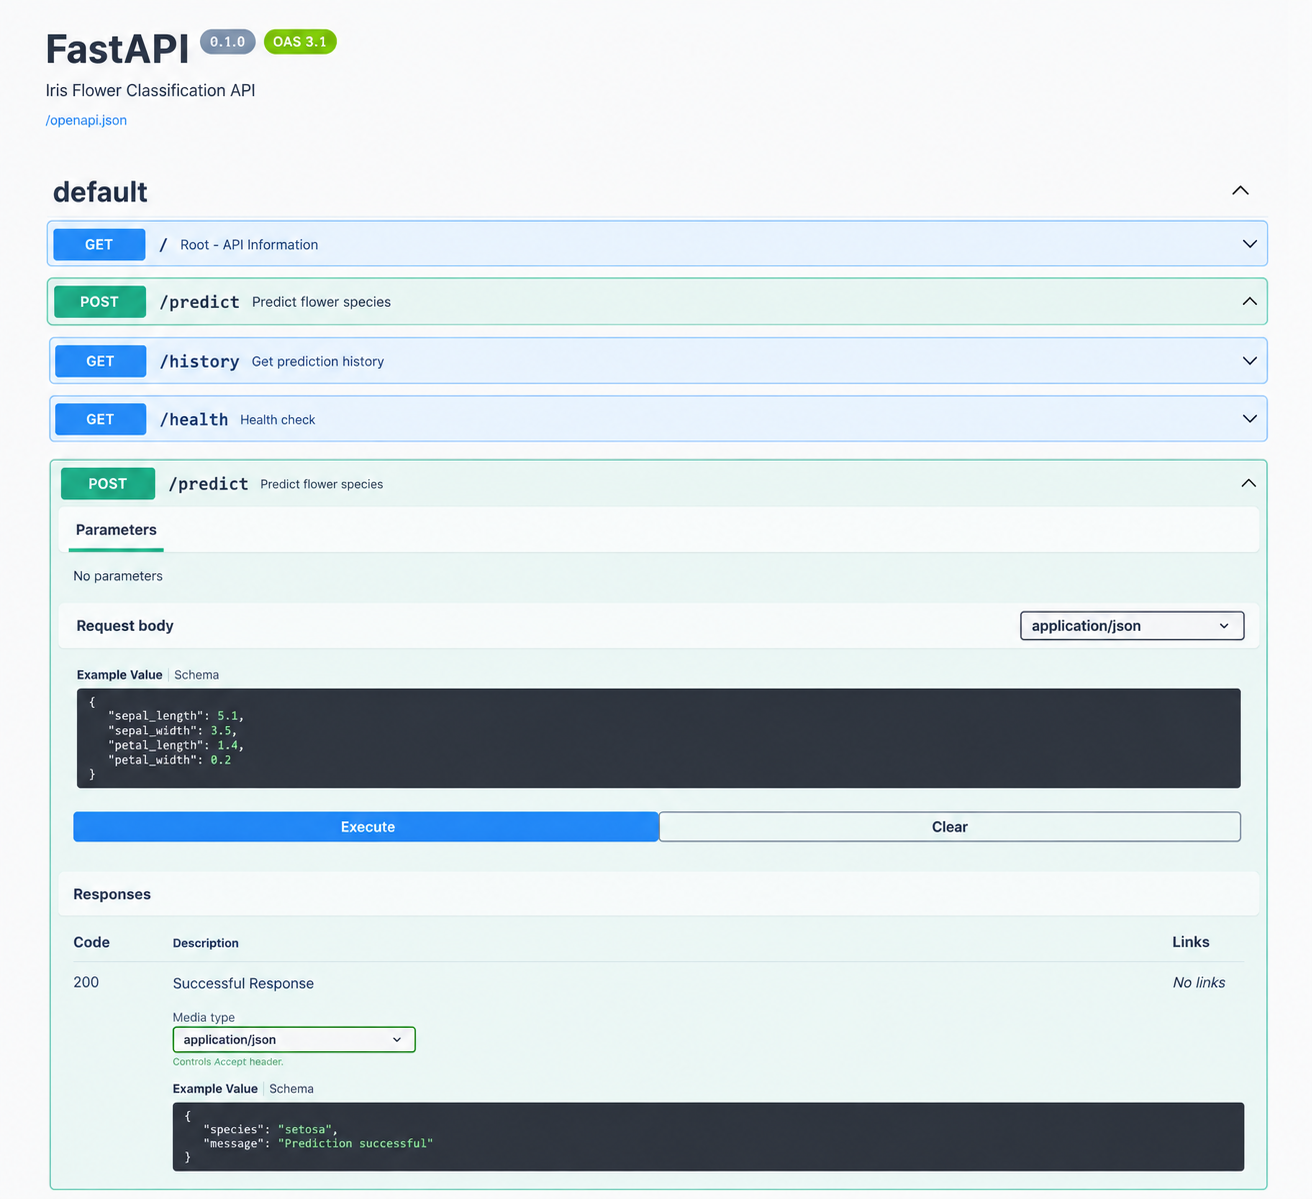
\includegraphics[width=0.6\textwidth]{images/api_predict.png}
	\caption{Kiểm thử API dự đoán thông qua Swagger UI}
	\label{fig:apipredict}
\end{figure}
	
	\noindent Trong quá trình kiểm thử, dữ liệu đầu vào được truyền dưới dạng JSON. Backend thực hiện kiểm tra dữ liệu, gọi mô hình SVM và trả về kết quả phân loại.
	
	\noindent Một phản hồi thành công có thể có dạng:
	\begin{lstlisting}[language={}, numbers=none, frame=single, basicstyle=\ttfamily\small]
		{6
			"input": {
				"sepal_length": 5.1,
				"sepal_width": 3.5,
				"petal_length": 1.4,
				"petal_width": 0.2
			},
			"prediction_id": 0,
			"predicted_class": "Iris-setosa"
		}
	\end{lstlisting}
	
	
	\noindent Kết quả trên cho thấy API đã tiếp nhận đúng bốn đặc trưng đầu vào và trả về nhãn dự đoán tương ứng. Qua đó kiểm chứng được sự kết nối giữa Frontend, FastAPI Backend và mô hình SVM.
	
	\subsection{Kiểm thử chức năng người dùng}
	
	\noindent Hệ thống người dùng được kiểm tra thông qua các thao tác đăng ký, đăng nhập và duy trì phiên đăng nhập.
	
	\subsubsection{Kiểm thử đăng ký tài khoản}
	
	\noindent Người dùng nhập tên đăng nhập và mật khẩu vào biểu mẫu đăng ký. Hệ thống kiểm tra tính hợp lệ của dữ liệu trước khi tạo tài khoản mới.
	
	\noindent Trường hợp tên đăng nhập chưa tồn tại, thông tin người dùng được ghi vào cơ sở dữ liệu. Nếu tên đăng nhập đã tồn tại, hệ thống trả về thông báo phù hợp và không tạo bản ghi trùng lặp.
	
	\subsubsection{Kiểm thử đăng nhập}
	
	\noindent Khi người dùng nhập thông tin đăng nhập, Backend thực hiện đối chiếu dữ liệu với thông tin đã lưu trong cơ sở dữ liệu.
	
	\noindent Nếu thông tin chính xác, hệ thống tạo phiên đăng nhập và cho phép người dùng tiếp tục sử dụng các chức năng được bảo vệ. Nếu thông tin không chính xác, hệ thống trả về thông báo lỗi tương ứng.
	
	\subsubsection{Kiểm thử quản lý phiên}
	
	\noindent Sau khi đăng nhập thành công, hệ thống duy trì thông tin phiên để xác định tài khoản đang sử dụng. Khi người dùng đăng xuất, phiên hiện tại được kết thúc nhằm ngăn việc tiếp tục sử dụng trạng thái đăng nhập cũ.
	
	\subsection{Kiểm thử lưu trữ dữ liệu}
	
	\noindent Một trong những chức năng được bổ sung trong quá trình hoàn thiện sản phẩm là khả năng lưu trữ dữ liệu hoạt động của người dùng vào cơ sở dữ liệu.
	
	\noindent Các thông tin có thể được ghi nhận bao gồm tài khoản người dùng, thời gian đăng nhập, dữ liệu đầu vào của quá trình dự đoán, kết quả dự đoán và thông tin về thời gian xử lý mô hình.
	
	\subsection{Kiểm thử lịch sử dự đoán}
	
	\noindent Sau khi thực hiện dự đoán, thông tin về kết quả được ghi nhận vào lịch sử tương ứng với tài khoản đang đăng nhập. Người dùng có thể xem lại các lần dự đoán trước đó thông qua chức năng lịch sử trên giao diện.
	
	\noindent Việc xây dựng lịch sử dự đoán giúp phân biệt giữa quá trình xử lý hiện tại và dữ liệu đã phát sinh trước đó, đồng thời tạo nền tảng cho các chức năng quản lý dữ liệu như xóa mềm, khôi phục hoặc xóa vĩnh viễn.
	
	\subsection{Kiểm thử thời gian chạy mô hình}
	
	\noindent Để đánh giá khả năng đáp ứng của hệ thống Web, thời gian xử lý mô hình được ghi nhận trong quá trình thực hiện dự đoán.
	
	\noindent Thời gian này được xác định trong khoảng thời gian hệ thống thực hiện quá trình suy luận với mô hình SVM. Giá trị được ghi nhận giúp theo dõi hiệu năng thực tế của mô hình khi được tích hợp vào Backend.
	
	\noindent Việc ghi nhận thời gian chạy không thay thế cho các chỉ số đánh giá độ chính xác của mô hình. Hai nhóm chỉ số có mục đích khác nhau: các chỉ số như Accuracy, Precision, Recall và F1-score đánh giá chất lượng phân loại, trong khi thời gian chạy phản ánh hiệu năng xử lý của hệ thống.
	
	\subsection{Đánh giá kết quả vận hành}
	
	\noindent Qua các thử nghiệm, hệ thống đã hoàn thành chuỗi xử lý từ tiếp nhận dữ liệu người dùng, kiểm tra dữ liệu, gọi mô hình SVM, trả kết quả dự đoán và lưu trữ thông tin vào cơ sở dữ liệu.
	
	\noindent Quá trình kiểm thử cho thấy các thành phần của hệ thống có thể phối hợp theo đúng luồng thiết kế:
	
	\begin{center}
		\textbf{Người dùng}
		$\rightarrow$
		\textbf{Web}
		$\rightarrow$
		\textbf{FastAPI}
		$\rightarrow$
		\textbf{SVM}
		$\rightarrow$
		\textbf{Kết quả}
		$\rightarrow$
		\textbf{Cơ sở dữ liệu}
	\end{center}
	
	\noindent Như vậy, sản phẩm không chỉ dừng lại ở việc xây dựng và đánh giá một mô hình học máy mà đã được mở rộng thành một hệ thống có khả năng tương tác với người dùng, cung cấp API, quản lý tài khoản và lưu trữ dữ liệu phục vụ quá trình vận hành.
	
	\subsection{Tổng kết chương 3}
	
	\noindent Chương 3 đã trình bày cách sử dụng và quá trình kiểm thử hệ thống \textbf{IRIS BOTANICA AI} sau khi mô hình SVM được tích hợp vào ứng dụng Web. Các chức năng được kiểm tra bao gồm nhập dữ liệu và dự đoán, kiểm thử API, đăng ký và đăng nhập tài khoản, quản lý phiên, lưu trữ dữ liệu và ghi nhận thời gian xử lý.
	
	\noindent Kết quả thực nghiệm cho thấy mô hình SVM có thể được kết nối với Web API và giao diện người dùng để tạo thành một quy trình hoàn chỉnh từ dữ liệu đầu vào đến kết quả phân loại. Đồng thời, việc tích hợp cơ sở dữ liệu giúp hệ thống có khả năng lưu trữ và quản lý dữ liệu phát sinh trong quá trình sử dụng.
	\newpage 
	\section{KẾT LUẬN VÀ HƯỚNG PHÁT TRIỂN}
	
	\subsection{Kết quả đạt được}
	


\noindent Sau quá trình nghiên cứu, xây dựng, thực nghiệm và triển khai, đề tài ``Hệ thống phân loại hoa Iris và triển khai vận hành trực tuyến IRIS BOTANICA AI'' đã hoàn thành các nội dung chính đề ra.

\noindent Về mặt học thuật, đề tài đã tìm hiểu và áp dụng thuật toán Support Vector Machine (SVM) với kernel tuyến tính để xây dựng mô hình phân loại ba loài hoa \textit{Setosa}, \textit{Versicolor} và \textit{Virginica} trên bộ dữ liệu Iris gồm 150 mẫu và 4 đặc trưng đầu vào. Dữ liệu được khảo sát, trực quan hóa và sử dụng để huấn luyện, kiểm thử và đánh giá mô hình thông qua các chỉ số Accuracy, Precision, Recall, F1-score và ma trận nhầm lẫn.

\noindent Về mặt triển khai, mô hình sau khi huấn luyện được lưu trữ và tích hợp vào Backend FastAPI. Hệ thống đồng thời xây dựng API dự đoán và API cơ sở dữ liệu, cho phép kết nối giữa mô hình, ứng dụng Web và cơ sở dữ liệu SQLite.

\noindent Đề tài cũng phát triển các chức năng quản lý người dùng, đăng ký, đăng nhập, lưu lịch sử đăng nhập và lịch sử dự đoán. Dữ liệu dự đoán được lưu trữ cùng thời gian thực thi, đồng thời hỗ trợ cơ chế xóa mềm, khôi phục và xóa vĩnh viễn nhằm tăng khả năng quản lý dữ liệu.

\noindent Cuối cùng, các thành phần được tích hợp thành hệ thống Web \textbf{IRIS BOTANICA AI}, cho phép người dùng đăng nhập, nhập thông số của mẫu hoa, gửi yêu cầu dự đoán và nhận kết quả trực tiếp trên trình duyệt. Qua đó, đề tài đã xây dựng được quy trình tương đối hoàn chỉnh từ \textbf{dữ liệu → mô hình học máy → API → cơ sở dữ liệu → giao diện Web}, thể hiện khả năng chuyển một mô hình học máy từ môi trường phát triển sang hệ thống có khả năng vận hành trực tuyến.

	
\subsection{Những hạn chế của đề tài}

\noindent Mặc dù đã hoàn thành các chức năng chính, hệ thống vẫn còn một số hạn chế:

\begin{itemize}[leftmargin=*]
	
	\item \textbf{Quy mô dữ liệu còn nhỏ:} Bộ dữ liệu Iris chỉ gồm 150 mẫu thuộc ba loài hoa, do đó khả năng tổng quát hóa của mô hình trong các bài toán thực tế còn hạn chế.
	
	\item \textbf{Đặc trưng đầu vào còn giới hạn:} Mô hình hiện sử dụng bốn đặc trưng hình thái cơ bản. Các thông tin như màu sắc, hình ảnh hoặc đặc điểm môi trường chưa được khai thác.
	
	\item \textbf{Phạm vi phân loại còn hẹp:} Hệ thống hiện chỉ phân loại ba lớp của bộ dữ liệu Iris và chưa được kiểm chứng trên nhiều loài thực vật khác.
	
	\item \textbf{Bảo mật còn ở mức cơ bản:} Hệ thống đã hỗ trợ tài khoản và phiên đăng nhập nhưng chưa triển khai đầy đủ các cơ chế như mã hóa mật khẩu chuyên dụng, phân quyền nhiều cấp hoặc xác thực bằng token.
	
	\item \textbf{Phụ thuộc vào môi trường triển khai:} Thời gian phản hồi và khả năng đáp ứng của hệ thống trực tuyến còn phụ thuộc vào tài nguyên máy chủ, kết nối mạng và môi trường vận hành.
	
	\item \textbf{Mô hình chưa được tối ưu sâu:} Đề tài tập trung vào SVM với Kernel tuyến tính và chưa thực hiện mở rộng việc tìm kiếm siêu tham số hoặc so sánh nhiều cấu hình mô hình.
	
\end{itemize}

\subsection{Hướng phát triển}

\noindent Từ những kết quả và hạn chế trên, hệ thống có thể tiếp tục phát triển theo các hướng sau:

\begin{enumerate}[leftmargin=*]
	
	\item \textbf{Mở rộng tập dữ liệu và số lượng loài:} Thu thập thêm dữ liệu từ nhiều nguồn và bổ sung các loài hoa khác nhằm tăng khả năng tổng quát hóa của hệ thống.
	
	\item \textbf{So sánh và tối ưu mô hình:} Bổ sung các mô hình như KNN, Decision Tree, Random Forest và các cấu hình SVM khác; đồng thời áp dụng Grid Search hoặc Random Search để lựa chọn siêu tham số phù hợp.
	
	\item \textbf{Nghiên cứu mô hình phi tuyến:} Thử nghiệm các Kernel như RBF hoặc Polynomial khi dữ liệu có cấu trúc phức tạp hơn.
	
	\item \textbf{Phát triển nhận dạng từ hình ảnh:} Cho phép người dùng tải ảnh hoa thay vì nhập thủ công các thông số. Hệ thống có thể kết hợp xử lý ảnh và mô hình học sâu để thực hiện nhận dạng trực tiếp.
	
	\item \textbf{Nâng cao bảo mật:} Bổ sung mã hóa mật khẩu, JWT hoặc OAuth2, phân quyền tài khoản và các cơ chế bảo vệ API khi triển khai trong môi trường thực tế.
	
	\item \textbf{Nâng cao khả năng giám sát:} Xây dựng Dashboard theo dõi người dùng, số lần dự đoán, phân bố kết quả, thời gian phản hồi và trạng thái hoạt động của hệ thống.
	
	\item \textbf{Tự động hóa triển khai:} Áp dụng CI/CD để tự động kiểm thử, xây dựng và triển khai hệ thống khi mã nguồn được cập nhật.
	
\end{enumerate}


	
	\subsection{Hướng phát triển}
	
	\noindent Từ những kết quả và hạn chế trên, hệ thống có thể tiếp tục được phát triển theo các hướng sau:
	
	\begin{enumerate}[leftmargin=*]
		
	
		\item \textbf{Mở rộng tập dữ liệu:} Thu thập thêm dữ liệu từ nhiều nguồn khác nhau nhằm tăng số lượng mẫu và tăng khả năng tổng quát hóa của mô hình.
		
		\item \textbf{Mở rộng số lượng loài hoa:} Bổ sung thêm các loài hoa khác để biến hệ thống từ bài toán phân loại ba lớp thành một hệ thống nhận dạng nhiều lớp.
		
		\item \textbf{So sánh nhiều mô hình học máy:} Bổ sung và đánh giá các mô hình như Logistic Regression, K-Nearest Neighbors (KNN), Decision Tree, Random Forest hoặc các cấu hình SVM khác nhau. Các mô hình có thể được đánh giá bằng cùng một tập dữ liệu và cùng hệ thống chỉ số nhằm tạo cơ sở cho việc lựa chọn mô hình phù hợp.
		
		\item \textbf{Tối ưu siêu tham số:} Áp dụng các phương pháp như Grid Search hoặc Random Search để tìm các tham số phù hợp cho SVM, đặc biệt là tham số $C$ và các tham số của Kernel khi mở rộng sang các mô hình phi tuyến.
		
		\item \textbf{Bổ sung mô hình phi tuyến:} Khi dữ liệu có cấu trúc phức tạp hơn, có thể nghiên cứu các Kernel như RBF hoặc Polynomial để so sánh với Kernel tuyến tính về khả năng phân loại và chi phí tính toán.
		
		\item \textbf{Phát triển hệ thống nhận dạng từ hình ảnh:} Một hướng phát triển quan trọng là cho phép người dùng tải ảnh hoa thay vì nhập thủ công bốn thông số. Hệ thống có thể sử dụng các kỹ thuật xử lý ảnh và mô hình học sâu để trích xuất đặc trưng trực tiếp từ hình ảnh.
		
		\item \textbf{Nâng cao bảo mật hệ thống:} Có thể bổ sung mã hóa mật khẩu, xác thực người dùng bằng JWT hoặc OAuth2, phân quyền tài khoản và các cơ chế bảo vệ API nhằm nâng cao độ an toàn khi triển khai thực tế.
		
		\item \textbf{Nâng cao khả năng giám sát hệ thống:} Có thể xây dựng Dashboard theo dõi số lượng người dùng, số lần dự đoán, tỷ lệ từng lớp dự đoán, thời gian phản hồi API và tình trạng hoạt động của mô hình.
		
		\item \textbf{Tự động hóa quá trình triển khai:} Trong các phiên bản tiếp theo, hệ thống có thể áp dụng CI/CD để tự động kiểm thử, xây dựng và triển khai ứng dụng mỗi khi mã nguồn được cập nhật.
		
		
	\end{enumerate}
	
	\subsection{Kết luận chung}
	
	\noindent Đề tài đã xây dựng được một quy trình tương đối đầy đủ từ nghiên cứu lý thuyết SVM, khảo sát dữ liệu, huấn luyện và đánh giá mô hình đến đóng gói, xây dựng API, tích hợp cơ sở dữ liệu và triển khai ứng dụng Web.
	
	\noindent Điểm quan trọng của đề tài không chỉ nằm ở kết quả phân loại hoa Iris mà còn ở việc thể hiện được toàn bộ vòng đời cơ bản của một mô hình học máy trong thực tế. Mô hình được xây dựng từ dữ liệu, đánh giá trước khi sử dụng, đóng gói thành tập tin, đưa vào Backend thông qua API, kết nối với cơ sở dữ liệu và cuối cùng được cung cấp cho người dùng thông qua giao diện Web.
	
	\noindent Thông qua quá trình thực hiện, đề tài giúp củng cố kiến thức về học máy, đặc biệt là thuật toán SVM, đồng thời tạo cơ hội tiếp cận với các kỹ thuật triển khai mô hình học máy trực tuyến. Sản phẩm \textbf{IRIS BOTANICA AI} là kết quả của quá trình kết hợp giữa lý thuyết học máy và kỹ thuật phát triển phần mềm, qua đó minh họa rõ hơn quá trình chuyển một mô hình học máy từ môi trường nghiên cứu thành một ứng dụng có khả năng vận hành thực tế.
	

	% ============================================================
	% PHỤ LỤC
	% ============================================================
	
	\newpage
	\section*{PHỤ LỤC}
	\addcontentsline{toc}{section}{PHỤ LỤC}
	
	\noindent
	Phần phụ lục trình bày các thành phần quan trọng được sử dụng trong quá
	trình xây dựng và vận hành hệ thống \textbf{IRIS BOTANICA AI}. Nội dung
	được tổ chức theo từng nhóm nhằm giúp người đọc dễ dàng theo dõi quá trình
	từ huấn luyện mô hình, xây dựng API, kết nối cơ sở dữ liệu đến vận hành
	ứng dụng Web.
	
	\noindent
	Toàn bộ mã nguồn của đề tài được nộp riêng kèm theo sản phẩm. Vì vậy,
	phần phụ lục chỉ trình bày các đoạn mã tiêu biểu và hướng dẫn cần thiết
	để kiểm tra, sử dụng và vận hành hệ thống.
	
	
	% ============================================================
	% PHỤ LỤC A
	% ============================================================
	
	
	\subsection*{Phụ lục A. Hướng dẫn khởi chạy hệ thống}
	\addcontentsline{toc}{subsection}{Phụ lục A. Hướng dẫn khởi chạy hệ thống}
	
	\noindent
	Phần này trình bày các bước cần thực hiện để khởi động hệ thống
	\textbf{IRIS BOTANICA AI} trên môi trường máy tính cục bộ.
	
	\subsubsection*{A.1. Chuẩn bị môi trưường}
	
	\noindent
	Trước khi khởi chạy hệ thống, cần chuẩn bị:
	
	\begin{itemize}[leftmargin=*]
		\item Python 3.12 hoặc phiên bản tương thích.
		\item Visual Studio Code hoặc môi trường lập trình Python tương đương.
		\item Các thư viện được khai báo trong tệp \text{requirements.txt}.
		\item Toàn bộ mã nguồn của dự án \text{SVM-IRIS}.
		\item Tệp mô hình đã huấn luyện \text{svm\_model.pkl}.
		\item Cơ sở dữ liệu \texttt{iris\_database.db}.
	\end{itemize}
	
	\subsubsection*{A.2. Mở thư mục dự án}
	
	\noindent
	Mở thư mục chứa dự án \texttt{SVM-IRIS} bằng Visual Studio Code.
	Kiểm tra để đảm bảo các tệp chính của hệ thống đã được đặt đúng vị trí.
	\begin{folderbox}[Cấu trúc thư mục dự án IRIS BOTANICA AI]
		
		\begin{forest}
			for tree={
				font=\small\ttfamily,
				grow'=0,
				child anchor=west,
				parent anchor=south west,
				anchor=west,
				l sep=5pt,
				s sep=2pt,
				edge path={
					\noexpand\path[draw]
					(!u.parent anchor) ++(3pt,0) |- (.child anchor);
				}
			}
			[IRIS-BOTANICA-AI
			[app.py]
			[TRAIN\_SVM.py]
			[evaluate\_models.py]
			[index.html]
			[database
			[connection.py]
			[user.py]
			[history.py]
			[prediction.py]
			[model.py]
			[model\_history.py]
			]
			[SQL]
			[images]
			[report]
			[Iris.csv]
			[svm\_model.pkl]
			[lda\_model.pkl]
			[knn\_model.pkl]
			[requirements.txt]
			[Procfile]
			[render.yaml]
			]
		\end{forest}
		
	\end{folderbox}
	
	\subsubsection*{A.3. Khởi động máy chủ FastAPI}
	
	\noindent
	Mở Terminal tại thư mục dự án và thực hiện lệnh:
	
	\begin{lstlisting}[language=bash,
		numbers=none,
		frame=single,
		basicstyle=\ttfamily\small]
		python -m uvicorn app:app --reload
	\end{lstlisting}
	
	\noindent
	Tham số \text{--reload} cho phép máy chủ tự động khởi động lại khi
	mã nguồn được thay đổi trong quá trình phát triển.
	
	\noindent
	Nếu khởi động thành công, Terminal sẽ hiển thị thông báo máy chủ đang
	chạy tại địa chỉ cục bộ.
	
newpage
	\newpage
	\subsubsection*{A.4. Kiểm tra hệ thống}
	
	\noindent
	Sau khi máy chủ được khởi động, mở trình duyệt và truy cập:
	
	\begin{center}
		\texttt{http://127.0.0.1:8000}
	\end{center}
	
	\noindent
	Để kiểm tra các API thông qua giao diện Swagger UI, truy cập:
	
	\begin{center}
		\texttt{http://127.0.0.1:8000/docs}
	\end{center}
	

	
	
	% ============================================================
	% PHỤ LỤC B
	% ============================================================
	
	
	\subsection*{Phụ lục B. Hướng dẫn sử dụng Web IRIS BOTANICA AI}
	\addcontentsline{toc}{subsection}{Phụ lục B. Hướng dẫn sử dụng Web IRIS BOTANICA AI}
	
	\noindent
	Phần này trình bày quy trình sử dụng sản phẩm từ khi người dùng truy cập
	hệ thống đến khi nhận được kết quả phân loại hoa Iris.
	
	\subsubsection*{B.1. Truy cập hệ thống}
	
	\noindent
	Người dùng truy cập địa chỉ Web của hệ thống
	\textbf{IRIS BOTANICA AI} bằng trình duyệt.
	
	\subsubsection*{B.2. Đăng ký tài khoản}
	
	\noindent
	Người dùng lựa chọn chức năng đăng ký và nhập thông tin tài khoản theo
	yêu cầu của hệ thống.
	
	\noindent
	Sau khi đăng ký thành công, thông tin người dùng được lưu vào cơ sở
	dữ liệu để phục vụ quá trình đăng nhập và quản lý lịch sử sử dụng.
	
	
	\subsubsection*{B.3. Đăng nhập}
	
	\noindent
	Người dùng nhập tên đăng nhập và mật khẩu đã đăng ký. Hệ thống kiểm tra
	thông tin với dữ liệu được lưu trong cơ sở dữ liệu.
	
	\noindent
	Nếu thông tin hợp lệ, người dùng được xác thực và có thể sử dụng các
	chức năng của hệ thống.
	
	\subsubsection*{B.4. Nhập thông số hoa Iris}
	
	\noindent
	Người dùng nhập bốn thông số hình thái của mẫu hoa:
	
	\begin{itemize}[leftmargin=*]
		\item Chiều dài đài hoa.
		\item Chiều rộng đài hoa.
		\item Chiều dài cánh hoa.
		\item Chiều rộng cánh hoa.
	\end{itemize}
	
	\noindent
	Các thông số này được sử dụng làm dữ liệu đầu vào cho mô hình SVM.
	
	
	\subsubsection*{B.5. Thực hiện dự đoán}
	
	\noindent
	Sau khi nhập đầy đủ dữ liệu, người dùng nhấn nút dự đoán. Giao diện Web
	gửi yêu cầu đến API \texttt{/predict}.
	
	\noindent
	API tiếp nhận dữ liệu, đưa dữ liệu vào mô hình SVM và trả về kết quả
	phân loại.
	
	\subsubsection*{B.6. Hiển thị kết quả}
	
	\noindent
	Kết quả dự đoán được hiển thị trực tiếp trên giao diện Web. Hệ thống
	có thể trả về một trong ba lớp:
	
	\begin{itemize}[leftmargin=*]
		\item \textit{Iris-setosa}.
		\item \textit{Iris-versicolor}.
		\item \textit{Iris-virginica}.
	\end{itemize}
	
	
	
	\subsubsection*{B.7. Xem lịch sử sử dụng}
	
	\noindent
	Sau khi thực hiện dự đoán, kết quả được lưu trữ để người dùng có thể
	xem lại lịch sử sử dụng của mình.
	

	
	% ============================================================
	% PHỤ LỤC C
	% ============================================================
	
	
	\subsection*{Phụ lục C. Hướng dẫn kiểm thử API}
	\addcontentsline{toc}{subsection}{Phụ lục C. Hướng dẫn kiểm thử API}
	
	\noindent
	Hệ thống cung cấp giao diện Swagger UI giúp kiểm tra trực tiếp các
	API mà không cần sử dụng thêm công cụ bên ngoài.
	
	\subsubsection*{C.1. Mở giao diện kiểm thử API}
	
	\noindent
	Truy cập:
	
	\begin{center}
		\texttt{http://127.0.0.1:8000/docs}
	\end{center}
	

	\subsubsection*{C.2. Kiểm thử API dự đoán}
	
	\noindent
	Chọn API:
	
	\begin{center}
		\texttt{POST /predict}
	\end{center}
	
	\noindent
	Sau đó chọn chức năng \text{Try it out} và nhập dữ liệu kiểm thử.
	
	\begin{lstlisting}[numbers=none,
		frame=single,
		basicstyle=\ttfamily\small]
		{
			"sepal_length": 5.1,
			"sepal_width": 3.5,
			"petal_length": 1.4,
			"petal_width": 0.2
		}
	\end{lstlisting}
	
	\noindent
	Sau khi nhấn \text{Execute}, hệ thống trả về kết quả dưới dạng JSON.
	
	\begin{lstlisting}[numbers=none,
		frame=single,
		basicstyle=\ttfamily\small]
		{
			"prediction_id": 0,
			"predicted_class": "Iris-setosa"
		}
	\end{lstlisting}
	
	
	\subsubsection*{C.3. Kiểm tra dữ liệu không hợp lệ}
	
	\noindent
	Có thể nhập dữ liệu không đúng kiểu hoặc bỏ trống trường dữ liệu để
	kiểm tra khả năng xác thực dữ liệu của API.
	
	\noindent
	FastAPI và Pydantic sẽ phát hiện dữ liệu không hợp lệ và trả về thông
	báo lỗi tương ứng.
	
	
	% ============================================================
	% PHỤ LỤC D
	% ============================================================
	
	\newpage
	\subsection*{Phụ lục D. Hướng dẫn kiểm tra cơ sở dữ liệu}
	\addcontentsline{toc}{subsection}{Phụ lục D. Hướng dẫn kiểm tra cơ sở dữ liệu}
	
	\noindent
	Cơ sở dữ liệu được sử dụng để lưu trữ các thông tin phát sinh trong quá
	trình sử dụng hệ thống.
	
	\subsubsection*{D.1. Kiểm tra thông tin người dùng}
	
	\noindent
	Sau khi đăng ký tài khoản, thông tin người dùng được lưu vào bảng
	tương ứng trong cơ sở dữ liệu.
	
	
	\subsubsection*{D.2. Kiểm tra lịch sử đăng nhập}
	
	\noindent
	Mỗi lần người dùng đăng nhập thành công, hệ thống ghi nhận thông tin
	lịch sử đăng nhập nhằm phục vụ quản lý và kiểm tra hoạt động của hệ thống.
	

	
	\subsubsection*{D.3. Kiểm tra lịch sử dự đoán}
	
	\noindent
	Khi người dùng thực hiện dự đoán, dữ liệu đầu vào và kết quả phân loại
	được lưu vào cơ sở dữ liệu.
	
	\noindent
	Thông tin này cho phép người dùng xem lại các lần dự đoán trước đó và
	giúp hệ thống quản lý lịch sử sử dụng.
	
	\subsubsection*{D.4. Đối chiếu dữ liệu giữa Web và cơ sở dữ liệu}
	
	\noindent
	Quá trình lưu trữ dữ liệu được kiểm tra bằng cách thực hiện một thao tác
	trên Web, sau đó kiểm tra lại bản ghi tương ứng trong cơ sở dữ liệu.
	
	\begin{center}
		\textbf{
			Người dùng
			$\rightarrow$
			Web
			$\rightarrow$
			API
			$\rightarrow$
			Cơ sở dữ liệu
		}
	\end{center}
	
	\noindent
	Cách kiểm tra này giúp xác nhận dữ liệu được truyền và lưu trữ đúng
	giữa các thành phần của hệ thống.
	
	
	% ============================================================
	% PHỤ LỤC E
	% ============================================================
	

	\subsection*{Phụ lục E. Cấu trúc thư mục sản phẩm}
	\addcontentsline{toc}{subsection}{Phụ lục E. Cấu trúc thư mục sản phẩm}
	
	\noindent
	Dự án được tổ chức thành các thành phần tương ứng với từng chức năng
	của hệ thống:
	\newpage 
	\begin{lstlisting}[language={},
		numbers=none,
		frame=single,
		basicstyle=\ttfamily\small]
		SVM-IRIS/
		│
		├── app.py
		├── TRAIN_SVM.py
		├── svm_model.pkl
		├── Iris.csv
		├── requirements.txt
		├── Procfile
		├── render.yaml
		├── index.html
		│
		├── images/
		│
		├── database/
		│   ├── connection.py
		│   ├── model.py
		│   └── ...
		│
		├── charts/
		│   └── confusion_matrix.py
		│
		└── iris_database.db
	\end{lstlisting}
	
	\noindent
	Trong đó:
	
	\begin{itemize}[leftmargin=*]
		\item \texttt{TRAIN\_SVM.py}: chương trình huấn luyện và đánh giá
		mô hình SVM.
		
		\item \texttt{svm\_model.pkl}: tệp lưu mô hình SVM đã huấn luyện.
		
		\item \texttt{app.py}: chương trình Backend và các API của hệ thống.
		
		\item \texttt{index.html}: giao diện Web của sản phẩm.
		
		\item \texttt{database/}: các thành phần kết nối và thao tác với
		cơ sở dữ liệu.
		
		\item \texttt{charts/}: các chương trình tạo biểu đồ đánh giá và
		trực quan hóa dữ liệu.
		
		\item \texttt{iris\_database.db}: cơ sở dữ liệu của hệ thống.
	\end{itemize}
	
	
	% ============================================================
	% PHỤ LỤC F
	% ============================================================
	
	
	\subsection*{Phụ lục F. Quy trình vận hành sản phẩm}
	\addcontentsline{toc}{subsection}{Phụ lục F. Quy trình vận hành sản phẩm}
	
	\noindent
	Toàn bộ hệ thống được vận hành theo quy trình từ mô hình học máy đến
	ứng dụng Web như sau:
	
	\begin{center}
		\textbf{
			Dữ liệu Iris
			$\rightarrow$
			Huấn luyện SVM
			$\rightarrow$
			Đánh giá mô hình
			$\rightarrow$
			Lưu mô hình
		}
	\end{center}
	
	\begin{center}
		\textbf{
			$\downarrow$
		}
	\end{center}
	
	\begin{center}
		\textbf{
			FastAPI
			$\rightarrow$
			API dự đoán
			$\rightarrow$
			Cơ sở dữ liệu
			$\rightarrow$
			Giao diện Web
		}
	\end{center}
	
	\begin{center}
		\textbf{
			$\downarrow$
		}
	\end{center}
	
	\begin{center}
		\textbf{
			Người dùng
			$\rightarrow$
			Nhập dữ liệu
			$\rightarrow$
			Dự đoán
			$\rightarrow$
			Lưu lịch sử
		}
	\end{center}
	
	\subsubsection*{F.1. Các bước vận hành}
	
	\begin{enumerate}[leftmargin=*]
		
		\item Chuẩn bị tập dữ liệu Iris và mã nguồn của dự án.
		
		\item Huấn luyện mô hình SVM với Kernel tuyến tính.
		
		\item Đánh giá hiệu quả của mô hình trên tập kiểm thử.
		
		\item Huấn luyện mô hình cuối cùng và lưu thành
		\texttt{svm\_model.pkl}.
		
		\item Khởi động máy chủ FastAPI.
		
		\item Kiểm tra API thông qua Swagger UI.
		
		\item Kết nối hệ thống với cơ sở dữ liệu.
		
		\item Truy cập giao diện Web IRIS BOTANICA AI.
		
		\item Đăng ký hoặc đăng nhập tài khoản.
		
		\item Nhập bốn thông số của mẫu hoa Iris.
		
		\item Gửi yêu cầu dự đoán.
		
		\item API gọi mô hình SVM và trả về kết quả.
		
		\item Hệ thống lưu thông tin cần thiết vào cơ sở dữ liệu.
		
		\item Người dùng có thể xem lại lịch sử sử dụng.
		
	\end{enumerate}
	
	\subsubsection*{F.2. Kết quả vận hành}
	
	\noindent
	Sau khi hoàn thành các bước trên, hệ thống có khả năng thực hiện đầy đủ
	chu trình từ dữ liệu đầu vào đến kết quả dự đoán trên giao diện Web.
	

	\noindent
	Địa chỉ sản phẩm trực tuyến:
	
	\begin{center}
		\url{https://iris-svm-api-4c5t.onrender.com/}
	\end{center}
	
	
	
	\noindent
	\textbf{Ghi chú:} Toàn bộ mã nguồn đầy đủ của sản phẩm được cung cấp
	riêng kèm theo báo cáo. Phần phụ lục có mục đích minh họa các thành phần
	quan trọng và cung cấp hướng dẫn kiểm tra, sử dụng và vận hành hệ thống.
	
	
	% Đổi tên tiêu đề mặc định của môi trường bibliography thành tiếng Việt
	\renewcommand{\refname}{TÀI LIỆU THAM KHẢO}
	\addcontentsline{toc}{section}{TÀI LIỆU THAM KHẢO}
	
	\begin{thebibliography}{99}
		
		\bibitem{scikit-learn}
		Học máy cơ bản, Tôn Thất Tú(2025) 
	
		\bibitem{iris-dataset}
		Fisher, R. A. (1936). 
		\textit{The use of multiple measurements in taxonomic problems}. 
		Annals of Eugenics, 7(2), 179-188.
		
		\bibitem{fastapi}2025
		Tiangolo (Sebastián Ramírez). (2018). 
		\textit{FastAPI framework, high performance, easy to learn, fast to code, ready for production}. 
		Trang chủ: \url{https://fastapi.tiangolo.com/}.
		
		\bibitem{github-pages}
		GitHub Documentation. (2024). 
		\textit{GitHub Pages Overview}. 
		Truy cập tại: \url{https://docs.github.com/en/pages}.
		
		\bibitem{render-docs}
		Render Cloud Documentation. (2024). 
		\textit{Deploying Python Web Services on Render}. 
		Truy cập tại: \url{https://render.com/docs}.
		
	\end{thebibliography}
	
	\end{document}